\section{The Proposed Method}
\subsection{Motivation}
Let the nominal frequency be $f_o$ and the actual system be at frequency $f$. The nominal time-period is given as \begin{align}
T_o &= \frac{1}{f_o}\nonumber\\
\intertext{Let the sinusoidal voltage signal be given as}
v(t) &= V_m\sin(2\pi f t +\phi)\nonumber\\
\intertext{In order to calculate the moving average voltage, we perform an integration of the signal over the nominal time period $T_o$. This integral will be zero if the system is at nominal frequency. If the system is at off nominal frequency then we will show that the integral is another sinusoidal signal with a frequency $f$ having an amplitude which is dependant on the system frequency.Therefore,}
& \frac{1}{T_o}\int\limits_t^{t+T_o}V_m \sin(2\pi f t +\phi)dt\nonumber\\
&= V_m sinc(f T_o)\sin(2\pi f t +\varphi)\nonumber\\
\intertext{Or}
v_{avg}(t) &= F_m\sin(2\pi f t + \varphi)\nonumber\\
\intertext{where $v_{avg}$ is a moving cycle average, and $F_m$ is the amplitude of the average voltage waveform given by,}
F_m &= V_m sinc(f T_o)\nonumber\\
\intertext{and $\varphi$ is given as}
\varphi &= \phi + \pi f T_o\nonumber
\intertext{Thus the system frequency can be evaluated by estimating $F_m$ and $V_m$ and solving the equation}
\label{maineqn}
\frac{F_m}{V_m} &= sinc(f T_o)
\end{align}
The frequency response of (\ref{maineqn}) is shown in \figurename \ref{frequency_response 1} taking nominal frequency value to be 50Hz.
\begin{figure}[!t]
\centering
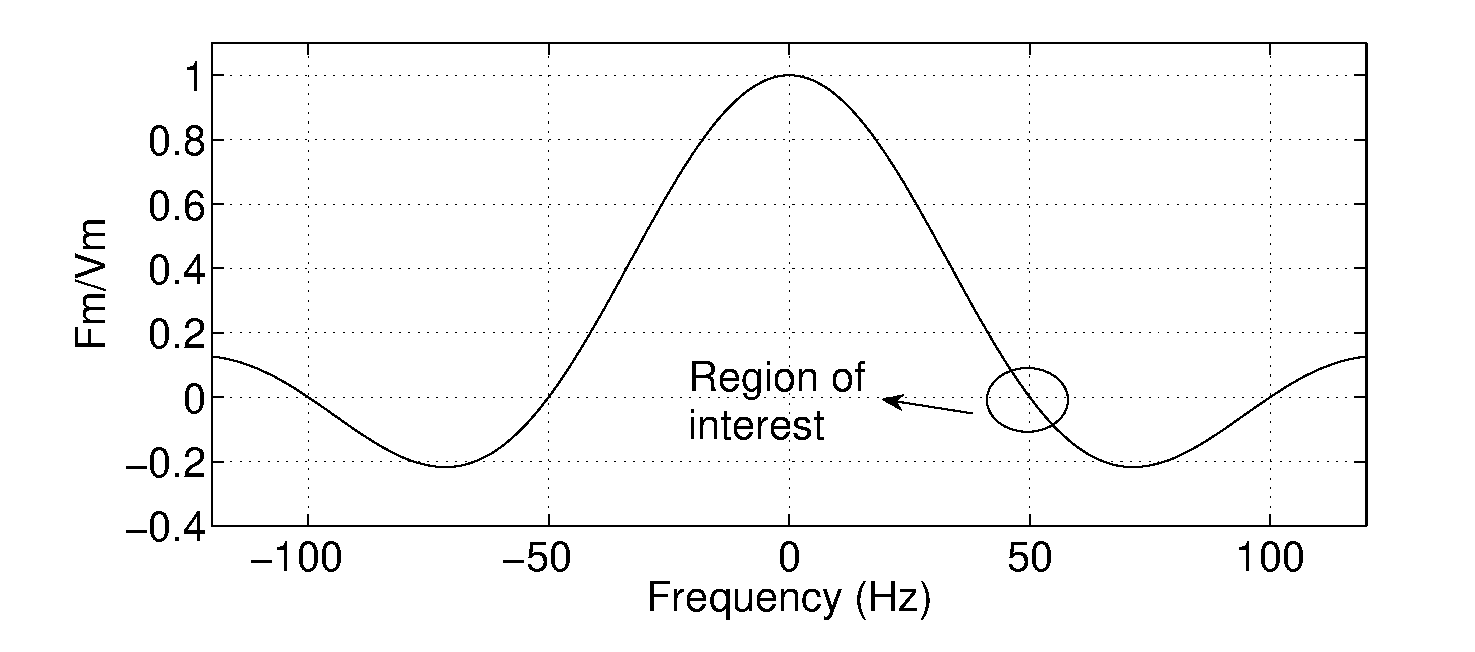
\includegraphics[height=1.1in,width=3.3in]{sincplot.eps}
\caption{Frequency response of \ref{maineqn}}
\label{frequency_response 1}
\end{figure}
\par Also further,
\begin{align}
 \frac{F_m}{V_m} &=\frac{\sin (\pi f_0T_0+\pi \vartriangle f_0T_0)}{\pi f_0T_0+\pi \vartriangle f_0T_0}\\
              &=\frac{\sin (\pi +\pi \vartriangle fT_0)}{\pi+\pi \vartriangle fT_0} 
 \intertext{Since $\vartriangle f$ is small  $\pi \vartriangle fT_0$ is close to zero. \newline Hence,}
\frac{F_m}{V_m} & = \frac{\sin(\pi +\pi \vartriangle fT_0)}{\pi+\pi \vartriangle fT_0)}\\
             & = - \frac{\sin(\pi \vartriangle fT_0)}{\pi+\pi \vartriangle fT_0}
\end{align}
It is to be noted that although $V_m$ is positive through out, $F_m$ is positive if $f<f_o$ and negative if $f>f_o$. Hence it can be concluded that in case of negative frequency deviation the voltage and the average voltage waveform are almost out of phase by $\pi$, and in the case of positive deviation they are almost entirely in phase, as shown in \figurename\ref{vAvv4951}.
\begin{figure}[!t]
\centering
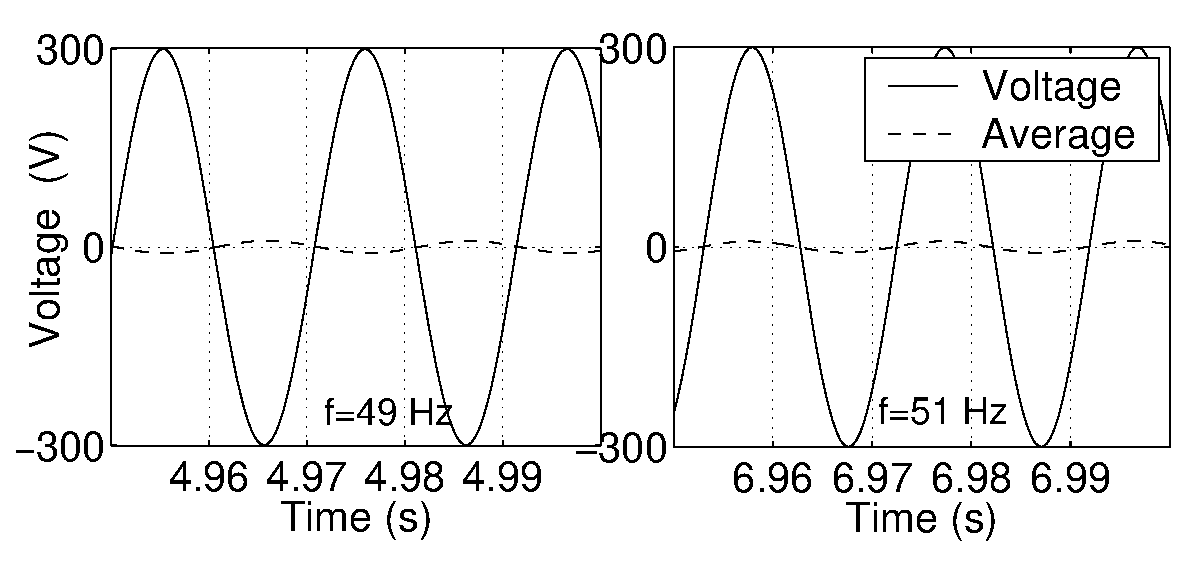
\includegraphics[height=1.3in,width=3.45in]{4951hz.eps}
\caption{Plot of Voltage and average voltage signal for 49 Hz and 51 Hz}
\label{vAvv4951}
\end{figure}
Therefore the computation of $F_m$ involves computation of both the magnitude and sign of $F_m$. The value of $|V_m|$ and $|F_m|$ can be computed using Discrete Fourier Transform as follows.
\subsubsection{Estimation of $V_m$}
Let the available signal be sampled at a frequency $f_s$ where
\begin{align}
\label{algo1}
\frac{f_s}{f_o}&=N
\end{align}
where N is the number of samples per cycle at nominal frequency, N being an integer. Let the voltage samples be given as $V_k$ where $k=[1,2,\dots]$. Now applying DFT on these samples we get
\begin{align}
V_c^w(m)&=\frac{2}{N}\sum_{k=w}^{N+w-1} v_k\cos(\frac{2\pi}{N}km)\nonumber\\
V_s^w(m)&=\frac{2}{N}\sum_{k=w}^{N+w-1} v_k\sin(\frac{2\pi}{N}km)\nonumber\\
\intertext{where $w$ is the window number. Our convention is that we associate the window number with the first sample in that window. From this we get a recursive update as}
\label{algo2}
V_c^{w+1}(m)&=V_c^w(m) + \frac{2}{N}(v_{w+N}-v_{w})\cos(\frac{2\pi}{N}wm)\\
\intertext{and similarly for sine component we have}
\label{algo3}
V_s^{w+1}(m)&=V_s^w(m) + \frac{2}{N}(v_{w+N}-v_{w})\sin(\frac{2\pi}{N}wm)\\
\intertext{from which we estimate $V_m$ as follows,}
\label{algo4}
V_m^w&=\sqrt{V_c^{w2}+V_s^{w2}}
\end{align}
\subsubsection{Calculation of $F_m$}
From the obtained samples of $v(t)$ we numerically integrate the signal using the trapezoidal rule of integration to get a moving average voltage signal. A recursive update for the integration is as follows,
\begin{equation}
\label{trap}
v_{avg,k}=v_{avg,k-1}+\frac{1}{N}\left[\frac{v_{k}+v_{k-1}}{2} - \frac{v_{k-N}+v_{k-N-1}}{2}\right]
\end{equation}
Now applying DFT on the samples generated from (\ref{trap}) we get the magnitude of $F_m$ i.e. $|F_m|$. But for one value of $|F_m|$ we get two possible values of $\Delta f$ as shown in \figurename\ref{zoom}.
\begin{figure}[!t]
\centering
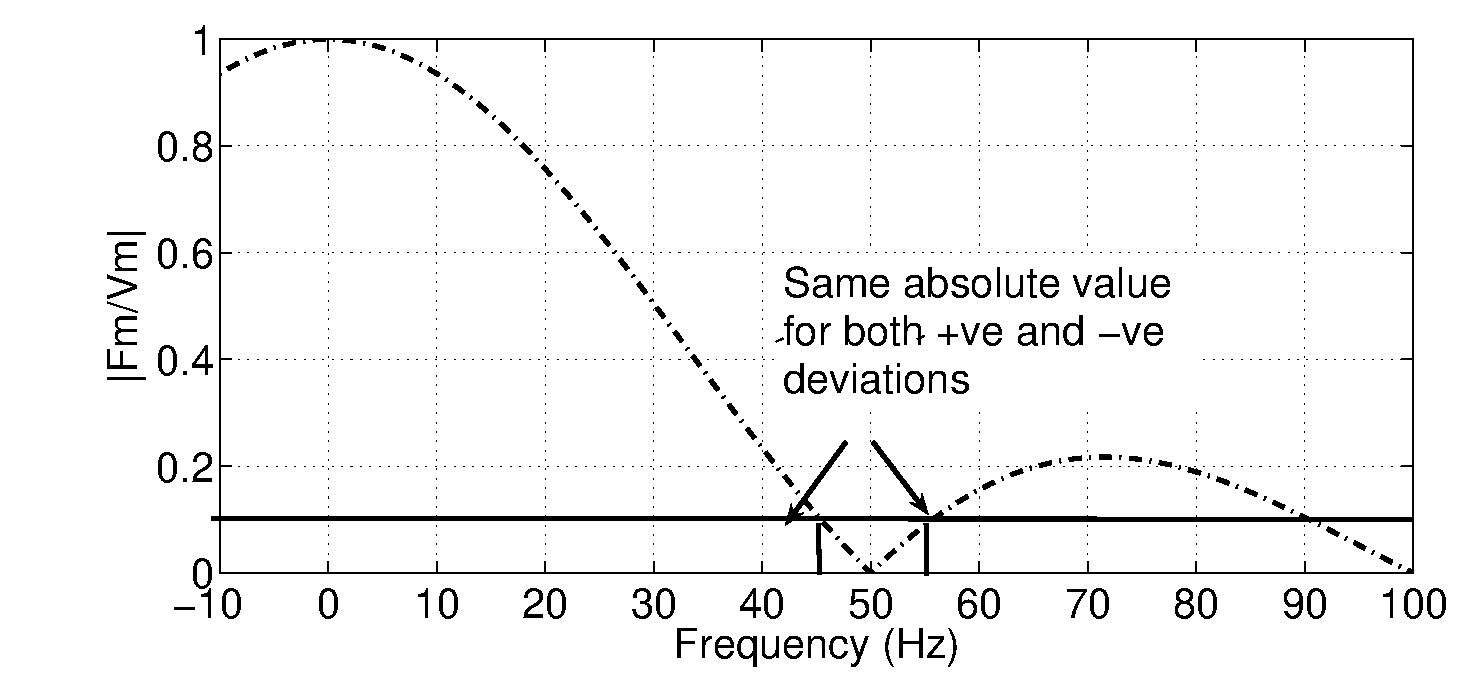
\includegraphics[scale=0.3]{abssincplot.eps}
\caption{Frequency response of  $|F_m/V_m|$}
\label{zoom}
\end{figure}
Therefore we need to consider the proper sign of $F_m$ before actually calculating frequency. In other words,we need to determine whether the voltage signal and its moving average signal are in-phase or out-of-phase. This can be done by first passing both the signals through a modified {\bf Schmitt trigger} to eliminate false triggering at zero crossings and then a comparator as implemented below.
 %\figurename \ref{scmidt51} and \figurename \ref{scmitt49}.
%\begin{figure}[!t]
%\centering
%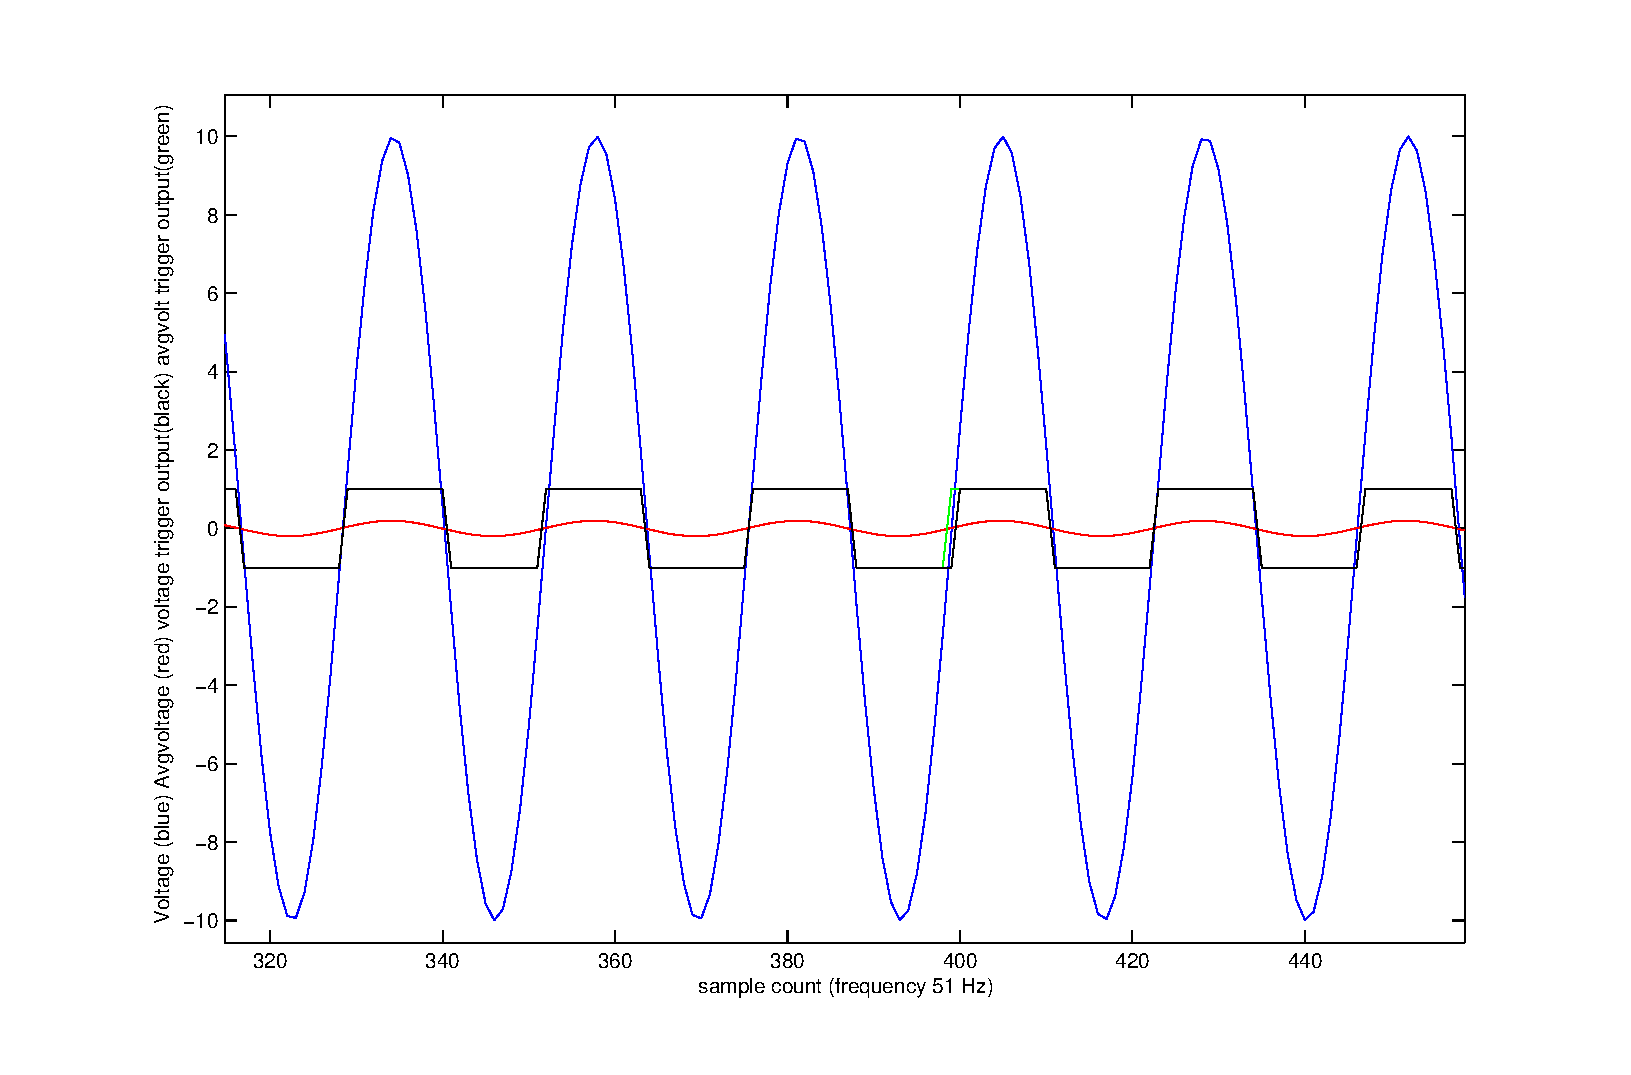
\includegraphics[width=3.2in]{scmitt51.eps}
%\caption{Schmitt trigger output Frequency 51 Hz}
%\label{scmitt51}
%\end{figure}

%\begin{figure}[!t]
%\centering
%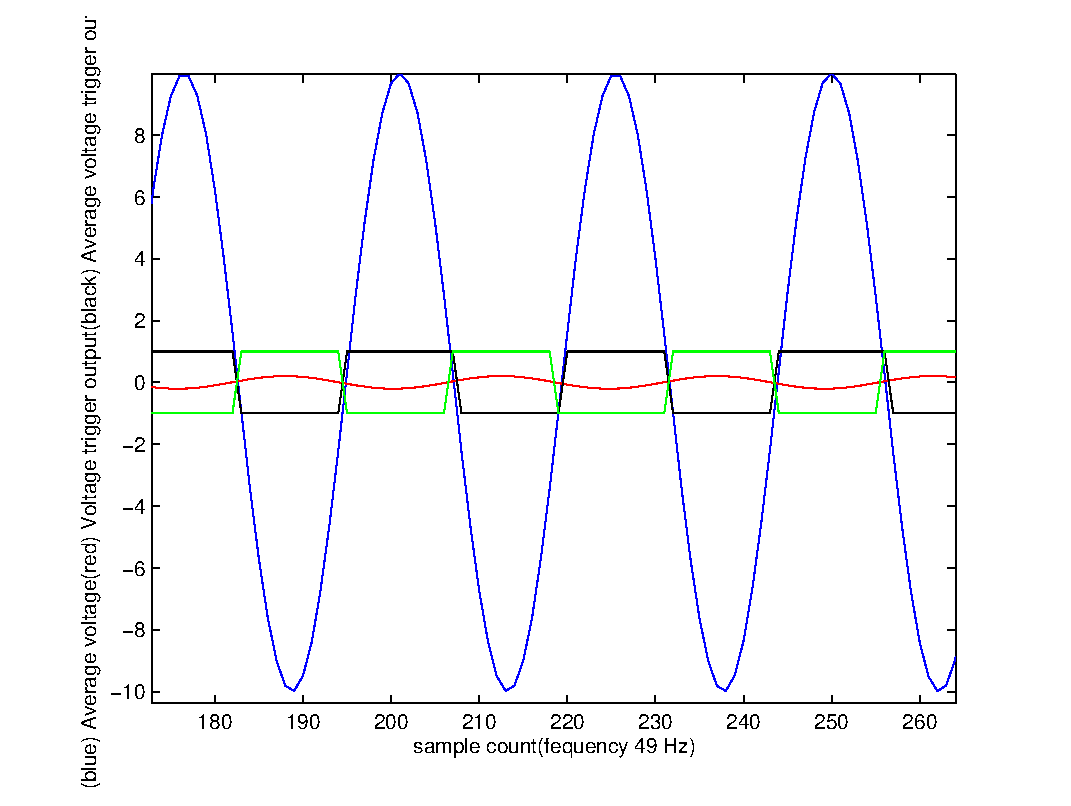
\includegraphics[width=3.0in]{scmitt49.eps}
%\caption{Schmitt trigger output Frequency 49 Hz}
%\label{scmitt49}
%\end{figure}
 Let the digital output of the voltage signal from the Schmitt trigger be $V_{sch}$ and that of the moving average voltage signal be $Avg_{sch}$. Then $F_m$ can be computed as follows:
\begin{align}
\label{sign}
F_m&=-V_{sch} Avg_{sch} |F_m|
\intertext{When $f < f_o$, then $v(t)$ and $v_{avg}(t)$ signals will be out-of-phase, so that $V_{sch} Avg_{sch}=-1$. Thus, $F_m$ would be given as}
F_m&=|F_m|\nonumber\\
\intertext{and when $f > f_o$, then $v(t)$ and $v_{avg}(t)$ signals will be in phase, so that $V_{sch} Avg_{sch}=1$. Thus, $F_m$ would be given as,}
F_m&=-|F_m|\nonumber\\
\intertext{Now taking the ratio of $F_m$ and $V_m$ we get,}
\frac{F_m}{V_m}&=sinc(f T_o)\nonumber\\
\end{align}from which frequency can be estimated.


\subsubsection{ Estimating Frequency }
Let $z$ be defined as follows,
\begin{flalign*}
z &= \frac{F_m}{V_m}\\
z &= sinc(f T_o)=\frac{\sin(\pi f T_o)}{\pi f T_o}\\
\intertext{Replacing f by $f_o+\Delta f$ we have}
z &= \frac{\sin(\pi {(f_o+\Delta f)} T_o)}{\pi {(f_o+\Delta f)} T_o}
\intertext{Now since $f_oT_o=1$ therefore we can further simplify the expression as}
z &= -\frac{\sin(\pi \Delta f T_o)}{\pi+\pi \Delta f T_o}\\
\intertext{Now since ${\Delta f}$ is small we can approximate $\sin(\pi \Delta f T_o)$ as $\pi \Delta f T_o$.Hence, it  can be further simplified as}
z &=-\frac{\pi \Delta f T_o}{\pi+\pi \Delta f T_o}
\end{flalign*}
Therefore we obtain the value of $\Delta f$ as
\begin{flalign}
\label{exp}
\Delta f &=-\frac{z}{1+z}f_o=-\frac{F_m}{V_m+F_m}f_o\\
\intertext{and hence the system frequency is given by}
\label{finalexp}
f &= f_o+\Delta f
\end{flalign}

\subsection{Model Algorithm}
The above idea can be summarized in as follows:
\begin{enumerate}
\item Obtain voltage (or current) samples from the system, The sampling frequency should be as given in (\ref{algo1}).
\item The sampled data should be fed into the DFT generator to calculate $V_m$ as mentioned in (\ref{algo2}), (\ref{algo3}), (\ref{algo4}).
\item The voltage samples is simultaneously fed to the integrator which then performs the averaging as mentioned in (\ref{trap}).
\item The average voltage samples are then fed to the DFT  which estimates $|F_m|$. $F_m$ is then calculated with proper sign using (\ref{sign}).
\item The computed $F_m$ and $V_m$ is then used to calculate frequency as per (\ref{exp}) and (\ref{finalexp}).
\end{enumerate}

\begin{figure}[!t]
\centering
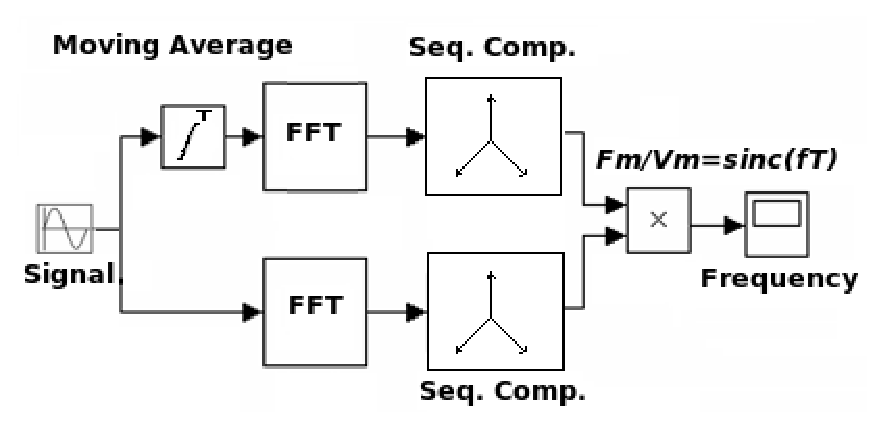
\includegraphics[height=1.1in,width=3.45in]{blockdiag.eps}
\caption{Block model diagram}
\label{blockdiag}
\end{figure}

\subsection{Estimation of rate-of-change of frequency}
\label{rate_estim}
Let the initial system frequency be $f=f_0+\Delta f$. Suppose at $t=\tau$,
frequency starts changing with rate $r$ and continues till $t=\delta$,
with $\delta > \tau$. If $U(t)$ is a unit function, $f(t)$ can be given by,
\begin{align*}
f(t)=&(f_0+\Delta f) + r(t-\tau) \left(U(t-\tau)-U(t-\delta)\right)\\
&+ r(\delta-\tau)U(t-\delta)
\end{align*}
Now for the time period $\tau < t < \delta$,the phase angle $\theta(t)$ given by ,
\begin{align*}
\theta(t) &= 2 \pi \Psi (t)\\
\Psi (t) &= \int_0^tf(t) dt\\
&=(f_0+\Delta f)t + \frac{r}{2}(t-\tau)^2\\
\intertext{Let complex voltage signal will be represented as,}
\bar{V}(t) &= V_me^{j\theta (t)} = [ V_m,\Psi(t) ]\\
&= [ V_m,(f_0+\Delta f)t + \frac{r}{2}(t-\tau)^2 ]
\intertext{Thus}
\bar{V}(t-\Delta t) &= [ V_m,(f_0+\Delta f)(t-\Delta t) +\frac{r}{2}(t-\Delta t-\tau)^2 ]
\intertext{where, $\Delta t$ is the time interval.\newline Defining,}
Z(t) &= \bar{V}(t-\Delta t)\bar{V}^\star(t)\\
Z(t) &= [ V_m^2,-(f_0+\Delta f)\Delta t+\frac{r}{2}(\Delta t-2(t-\tau))\Delta t ]\\
&= [ V_m^2,(-r\Delta t) t-(f_0+\Delta f)\Delta t\\
&+ r(\Delta t)\tau+\frac{r}{2}(\Delta t)^2 ]\\
\intertext{Hence, the obtained signal $Z(t)$ is oscillating with frequency $r\Delta t$ and has magnitude $V_m^2$. Since $r$ is expected to be very small, frequency of $Z(t)$ is very close to $0$. Hence, we frequency shift this signal by $f_0$, by simply multiplying it by $<1,f_0t>$.Thus,}
Z_{shift}(t) &= [ V_m^2,(f_0 -r\Delta t) t-(f_0+\Delta f)\Delta t\\
&+ r(\Delta t)\tau+\frac{r}{2}(\Delta t)^2 ]
\end{align*}
We can use above mentioned frequency estimation technique to estimate $r\Delta t$ and
hence, $r$.

\subsection{Oscillations in DFT response}
When considering a single phase signal it can be shown that the DFT response i.e. $|V_m^w|$ and $|F_m^w|$ will be oscillatory. These oscillations are because of the presence of a higher frequency components. This is evident from the analysis presented in \ref{DFToscillation} It is also shown how these oscillations can be removed by using all the three phases for estimating magnitudes $|V_m^w|$ and $|F_m^w|$.


\subsection{Computations for unbalanced systems}
For unbalanced system we can directly use SC DFT as mentioned in \cite{phadkethorp}. For unbalanced system, a recursive update can be used which is given in \ref{rec_update} . Or other wise we can use DFT SC, i.e. we shall first apply DFT on the voltage samples and construct the phasors. Then we extract the positive sequence components from these phasors.
\begin{align*}
V_A=V_{As}+jV_{Ac}\\
V_B=V_{Bs}+jV_{Bc}\\
V_C=V_{Cs}+jV_{Cc}
\end{align*}
Then we can extract the positive sequence components as follows,
\begin{align*}
V_A^+&=\frac{1}{3}(V_{As}+aV_{Bs}+a^2V_{Cs}+j(V_{Ac}+aV_{Bc}+a^2V_{Cc}))\\
V_B^+&=\frac{1}{3}(V_{Bs}+aV_{Cs}+a^2V_{As}+j(V_{Bc}+aV_{Cc}+a^2V_{Ac}))\\
V_C^+&=\frac{1}{3}(V_{Cs}+aV_{As}+a^2V_{Bs}+j(V_{Cc}+aV_{Ac}+a^2V_{Bc}))
\end{align*}

\subsection{Computations for single phase systems}
In single phase systems,as explained before, there will be oscillations which can only be avoided by using three phase information. Therefore for single phase analysis the other three phases should be constructed by giving the phasor at hand a +/- 120 degree shift. In discrete domain, however to get a +$\frac{2\pi}{3}$ shift the $(k-\frac{N}{3})^{th}$ sample should be considered and for a -$\frac{2\pi}{3}$ shift  the $(k-\frac{2N}{3})^{th}$ sample. Hence, considering the voltage samples available at hand as the A phase voltage, the other phases can be constructed as follows.
\begin{align*}
v_B^k&=v_A^{k-\frac{N}{3}}\\
v_C^k&=v_A^{k-\frac{2N}{3}}
\end{align*}
Now since the system is at offnominal frequency therefore the $(k-\frac{N}{3})^{th}$ would not give the required $\frac{2\pi}{3}$ phase shift. So evidently the three phase system obtained would be unbalanced in phase. Therefore we need to take the SCDFT or the DFTSC and then pass the balanced phases to the blackbox containing the algorithm for frequency estimation.

\subsection{Time response}
For full cycle DFT the time required to latch on to a value is one cycle. So, in estimating $V_m$ we have one cycle delay in measurement. Again while we integrate to calculate the moving average we have one cycle delay. Therefore when we calculate $F_m$ we have another one cycle delay. So, measurement of $F_m$ will take in total two cycles to latch on. Therefore the estimated value of frequency will also take two cycles to latch on.

\subsection{Frequency Response} The frequency response of the system is a {\bf sinc} curve, in the form of ${\bf sinc(fT_o)}$ which is depicted in the \figurename\ref{frequency_response 1}. It is evident that the higher frequency components are attenuated. This is the inherent advantage of the method. However, from the frequency response curve it is clear that the performance of the method will be better in the presence of high frequency components if the lobes in the frequency response curve are attenuated. This can be done by:
\begin{itemize}
\item Increasing the time of integration.
\item Sensitivity Enhancement.
\item Integrating twice in which case we get the frequency response as ${\bf [sinc(fT_o)]^2}$.
\end{itemize}
Let us explore each possibilities one by one.
\subsubsection{Increasing the time of Integration}
By increasing the time of integration we indeed found out that the higher frequency lobes in the frequency response are  getting attenuated and we get the following curve,
\begin{figure}[!t]
\centering
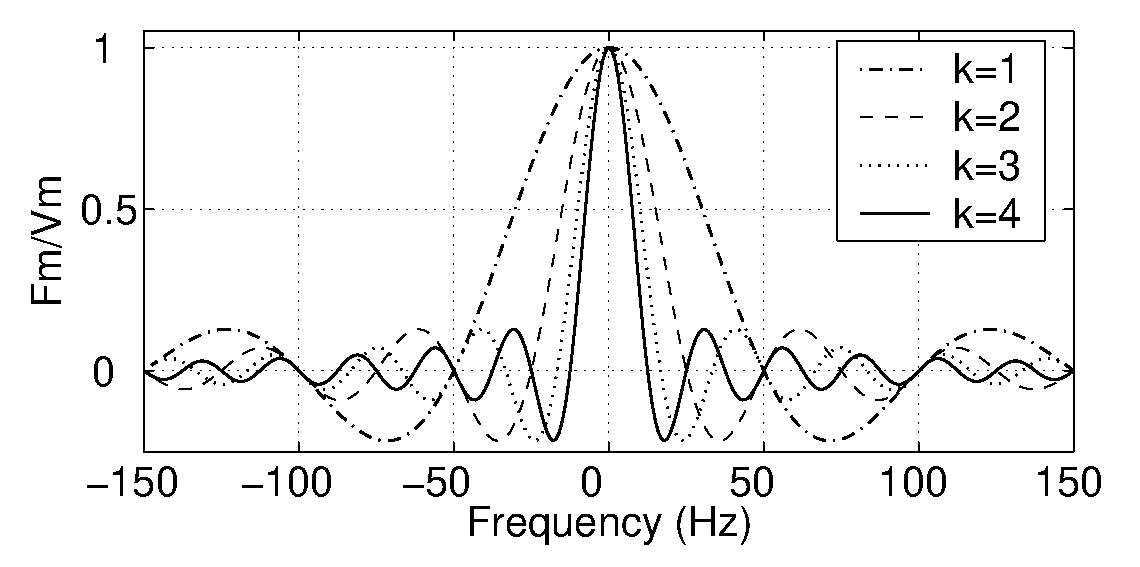
\includegraphics[scale=0.3]{diffksinc.eps}
\caption{Frequency response with different integration periods}
\label{frequency_response_vark}
\end{figure}

\figurename\ref{frequency_response_vark} has four plots. If we consider a variable {\bf k} as the number of cycles over which the averaging is done, then the blue plot is for $k=1$, red for $k=2$, green for $k=3$, and black for $k=4$. Therefore we see that at higher values of k the lobes at higher frequencies get more attenuated and the result improves. In the time domain, doing the integration over $k^{th}$ complete cycle will give
\begin{align*}
\frac{1}{kT_o}\int\limits_t^{t+kTo}V_m \sin(2\pi f t +\phi)dt\\
=V_m sinc(kf T_o)\sin(2\pi f t +\varphi)
\end{align*}
Hence increasing the time of integration also changes the frequency response. The new response now is ${\bf sinc(kfT_o)}$
However, it has been seen that with increasing the time of integration i.e. with increasing $k$ the tendency to overestimate the frequency value also increases. This is illustrated in \figurename\ref{vark}.
\begin{figure}[!t]
\centering
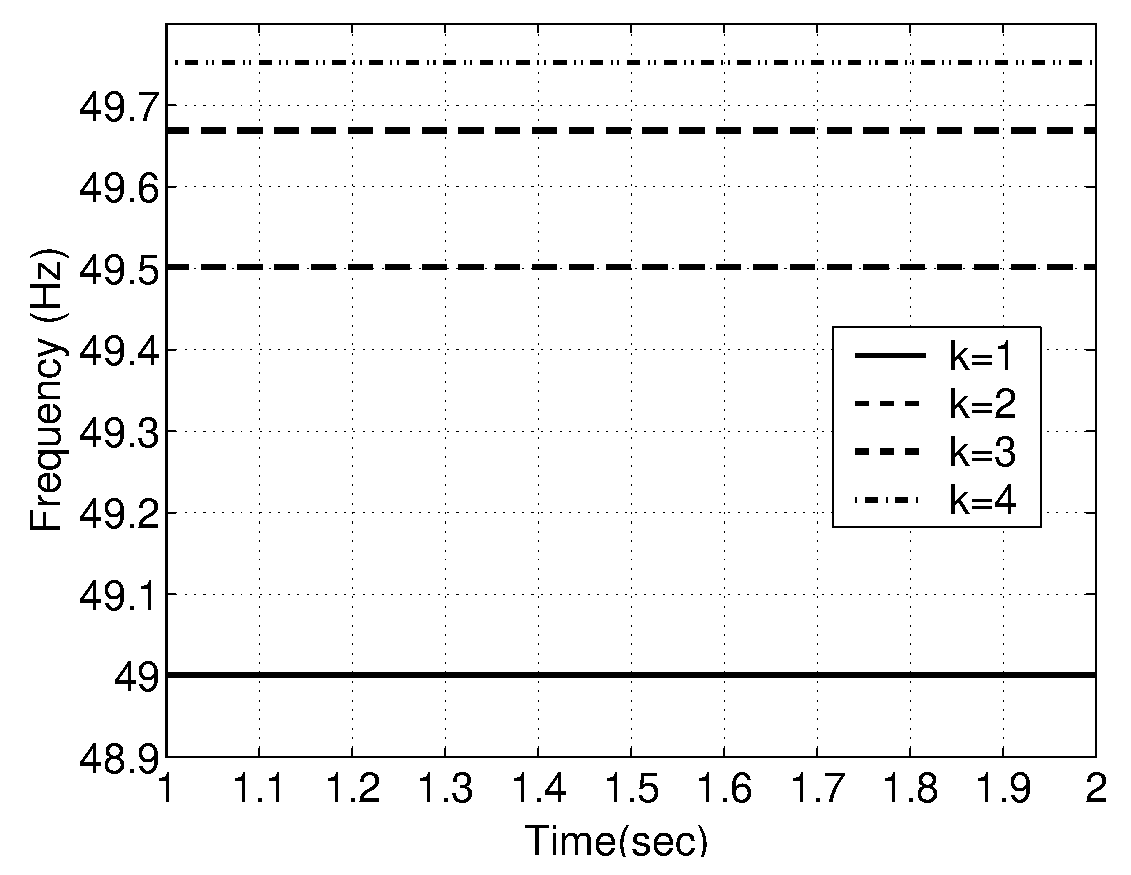
\includegraphics[scale=0.3]{overunderestimatenoshift}
\caption{Over estimation caused due to different integration periods}
\label{vark}
\end{figure}
\subsubsection{Sensitivity Enhancement}
\label{sens_enhance}
{\bf Sensitivity} of the method is directly dependant on the slope of the frequency response curve at the nominal frequency. So the motivation would be to increase the slope of the frequency response curve at around the nominal frequency. But although increasing the period of integration from ${\bf T_o}$ to ${\bf kT_o}$ improves the {\bf Harmonics and higher frequency components rejection} the noise filtering property of the system does not change as the slope of the new frequency response curve obtained i.e. ${\bf sinc(k f T_o)}$is same at the nominal frequency.
\begin{equation}
|\frac{d}{df}sinc(k f T_o)|=f_o    ~~~~\forall k
\end{equation}
Therefore it is evident that simply increasing the window size will not improve the estimation. Therefore, what we need is to increase the window size and simultaneously increase the slope of the curve at 50 Hz. Looking at the frequency response for different values of $k$ as in \figurename\ref{frequency_response_vark} we see that although the slope at $f=f_o$ is same the curves do successively attain higher slopes with increasing k. We can therefore use the high slopes at around $f_o$ by shifting the curve by required amount. Intuitively this is found possible if we can synthesize a function such as
\begin{align}
\label{newsignal}
v(t)&=V_m\sin(2\pi (f-(1-\frac{1}{k})f_o)t+\phi)
\intertext{where k is the number of cycles over which the averaging is done. On integrating over $kT_o$}
V_{avg}&=\frac{1}{kT_o}\int\limits_t^{t+kTo}V_m \sin(2\pi (f-(1-\frac{1}{k})f_o) t +\phi)dt\nonumber\\
V_{avg}&=V_m sinc(k(f-(1-\frac{1}{k})f_o) T_o)\sin(2\pi f t +\varphi)\nonumber
\end{align}
By taking the derivative at $f = f_o$ it is seen that
\begin{equation}
\frac{d}{df}sinc(k(f-(1-\frac{1}{k})f_o) T_o)=-\frac{k}{f_o}
\end{equation}
Therefore as we increase k the slope indeed increases as shown in \figurename\ref{shifted_response}
\begin{figure}[!t]
\centering
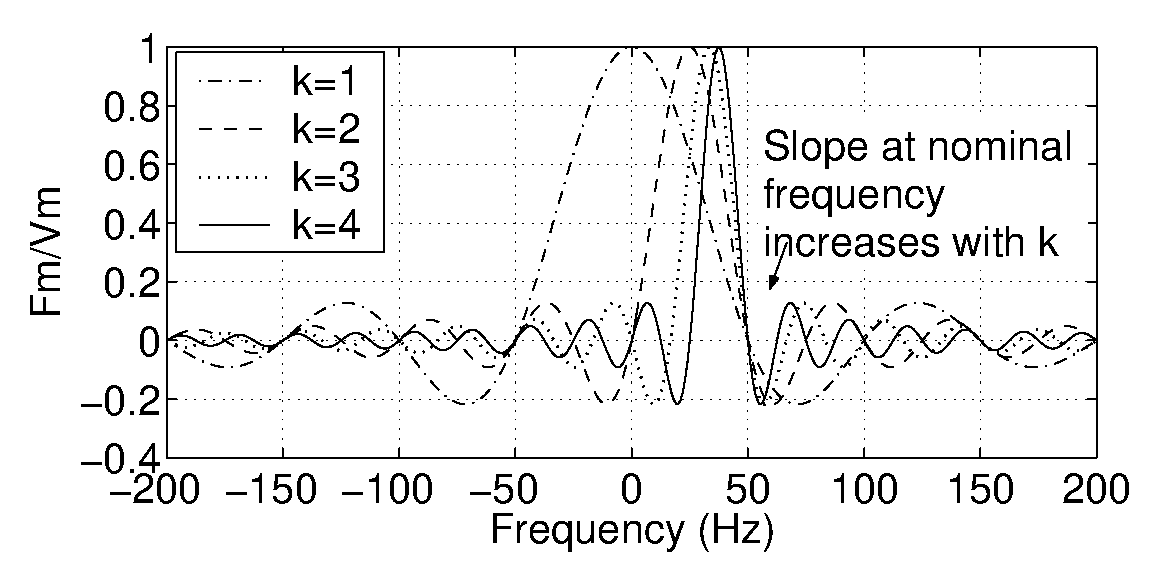
\includegraphics[height=1.1in,width=3.45in]{shiftksinc.eps}
\caption{Frequency response of shifted sinc curves for different integration periods}
\label{shifted_response}
\end{figure}
Thus with successively increasing k the slope at nominal frequency increases and hence increasing the noise rejection property. And also from actual computer generated samples, the result was confirmed that in presence of noise the output is much more stable, as shown in \figurename \ref{varknoise}
\begin{figure}[!t]
\centering
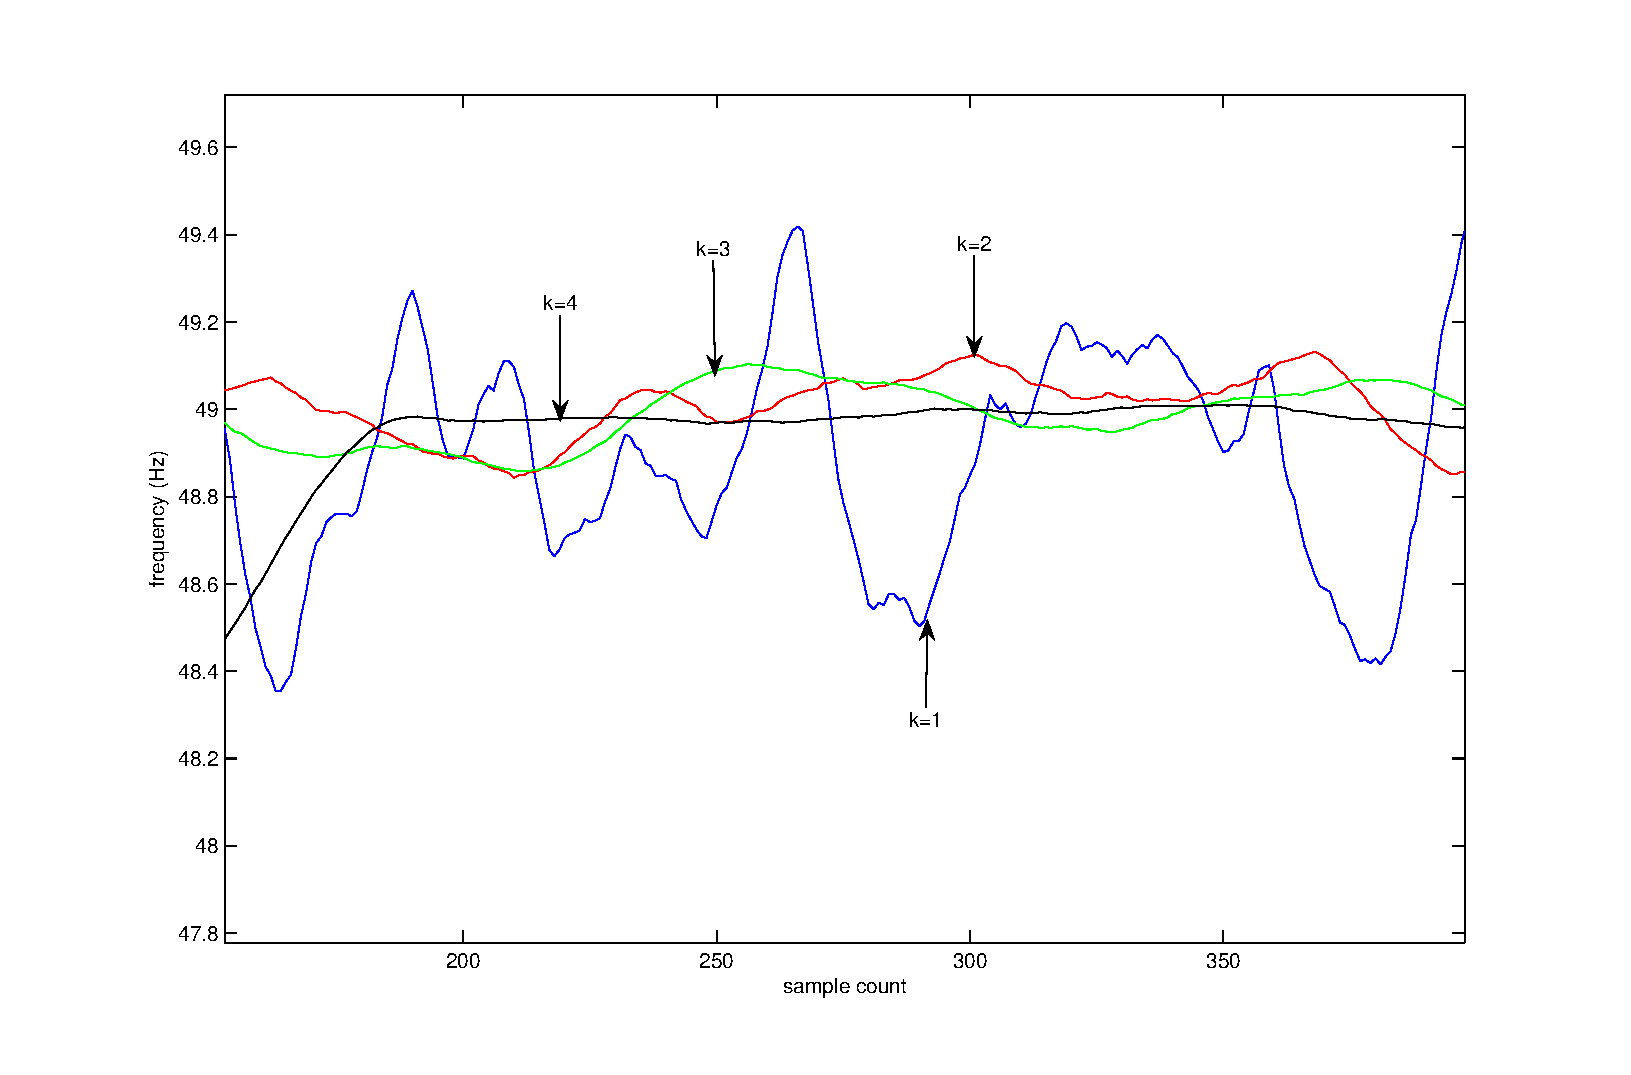
\includegraphics[height=1.1in,width=3.45in]{noiseestimateshifted}
\caption{Plot for estimated frequency in presence of noise}
\label{varknoise}
\end{figure}

Synthesizing the composite signal from the original one is explained below. In time domain, the signal that is required is,
\begin{align}
\label{synth1}
v(t)&=V_m\sin(2\pi (f-(1-\frac{1}{k})f_o)t+\phi)
\intertext{Expanding,}
v(t)&=V_m\left[\sin(2\pi f t + \phi)\cos(2\pi(1-\frac{1}{k})f_o t)\right]\nonumber\\
&-\left[\cos(2\pi f t +\phi)\sin(2\pi(1-\frac{1}{k})f_o t)\right]\nonumber
\end{align}
The expression ${\bf \sin(2\pi f t +\phi)}$ is directly obtained from the signal itself. We can simply multiply it with the expression ${\bf \cos(2\pi(1-\frac{1}{k})f_o t)}$. However to generate the ${\bf\cos(2\pi f t +\phi) }$ expression, we can take the help of the other two phases, i.e. if
\begin{align*}
v_a(t)&=V_m\sin(2\pi f t + \phi)\\
v_b(t)&=V_m\sin(2\pi f t + \phi - \frac{2\pi}{3})\\
v_c(t)&=V_m\sin(2\pi f t + \phi + \frac{2\pi}{3})
\end{align*}Therefore, in this case,
\begin{align}
\label{synth2}
V_m\cos(2\pi f t +\phi)&=\frac{v_c(t)-v_b(t)}{\sqrt{3}}
\end{align}

Similarly repeating the above process it can be done for other phases as well. Once the quadrature component for each phases are obtained the desired signal can be easily generated.However, as mentioned before, the algorithm has a tendency to overestimate for increasing values of $k$. This is illustrated in \figurename\ref{vark2}.
\begin{figure}[!t]
\centering
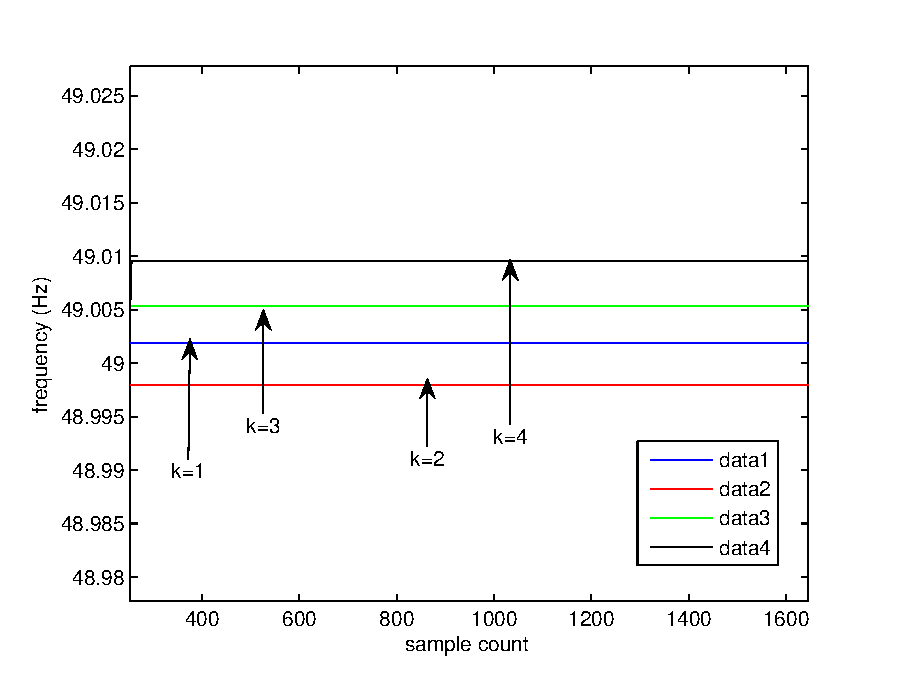
\includegraphics[width=3.0in]{overunderestimateshifted}
\caption{Plot for estimated frequency for (\ref{newsignal})}
\label{vark2}
\end{figure}
\footnote{If the shifted signal is used then with higher values of $k$, N should also be increased, or we can define N as $N=kN$.}
\subsubsection{Integrating two times}
In this case, the signal is averaged out two times. The frequency response becomes ${\bf [sinc(fT_o)]^2}$ and the lobes at higher frequencies are highly attenuated, as illustrated in \figurename\ref{squareshift}
\begin{figure}[!t]
\centering
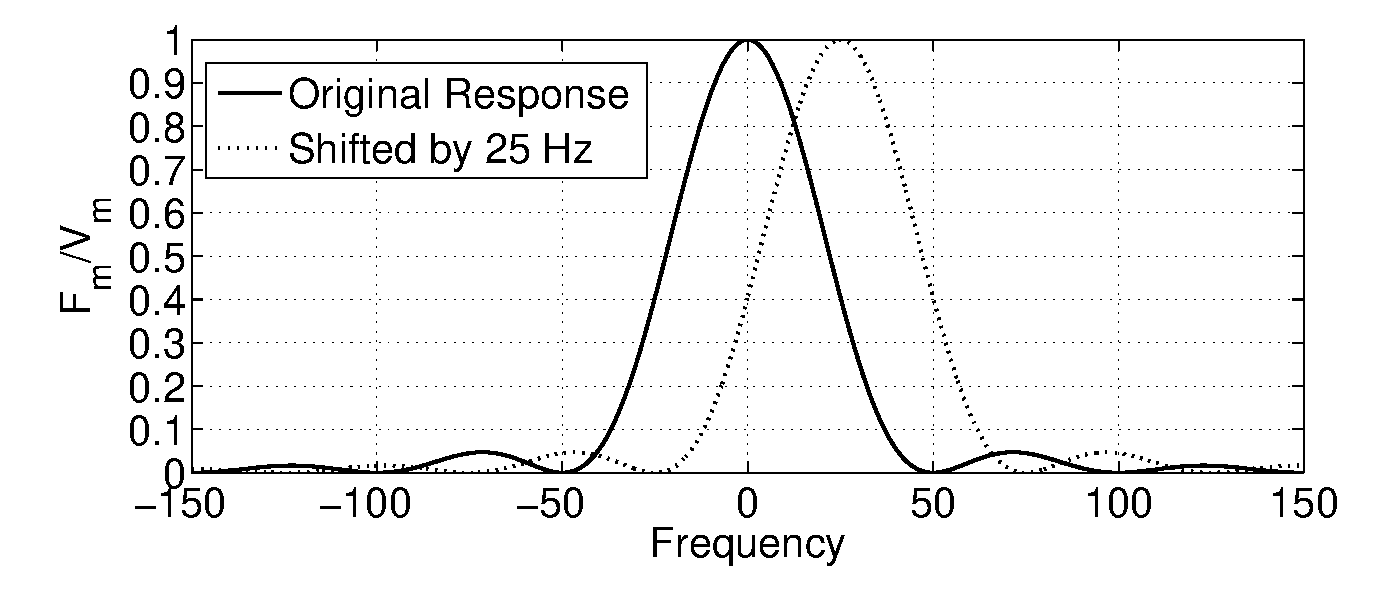
\includegraphics[width=3.0in]{squareshift}
\caption{Frequency response after averaging out two times}
\label{squareshift}
\end{figure}
However, it is seen that the slope of the frequency response is zero at 50 Hz, hence deteriorating the noise filtering property. Hence to remedy this the curve can be shifted (refer \figurename\ref{squareshift}). But the problem here is that with shifting, harmonic rejection becomes poor. Therefore in comparison with the previous method (i.e. increasing integration time) this method is not so efficient.

\subsection{Effect of introducing anti aliasing filters in the system}
Anti aliasing filters can also be integrated into the system. If an anti aliasing filter of cutoff frequency half of the sampling frequency be introduced in the system, then the higher frequency components would be reduced and in the algorithm  the $k$ value could be kept to unity. This will further reduce errors in estimation as higher $k$ values will lead to overestimation of frequency.

\subsection{Time Response for the shifted signal}
Time response of the shifted signal would be different from the original one. If the integration period is over $k$ complete cycles then the delay in measurement would be $2k$. In case we do not do the shifting, then an integration over $k$ cycles will give $k+1$ cycle delay in measurement. Therefore it is seen that with increasing $k$ accuracy increases in presence of noise but at the sacrifice of time. However this can be remedied by introducing a {\bf adaptive window hugging and minimum variance tracking} technique as mentioned below.
\subsubsection{Adaptive Window Hugging and minimum variance tracking technique}
A recursive update for mean and variance of the estimated frequency values is developed as follows
\begin{align*}
\mu_{w+1} &= \mu_w + \left[\frac{f_{w+1}-f_{w-N+1}}{N}\right]\\
\sigma^2_{w+1} &= \sigma^2_{w} + \left[\frac{f^2_{w+1} + f^2_{w-N+1}}{N}\right] - (\mu^2_{w+1} - \mu^2_{w})
\end{align*}
From this we can keep a track of the standard deviation of the frequency values. Therefore, we concurrently run three or four processes for different values of $k$, and keep a track of the standard deviation of the frequency values. The sample having minimum standard deviation would be picked up and given as the output.

\subsection{The Modified Algorithm}
Incorporating the above techniques we can device an algorithm as follows.
\begin{itemize}
\item First the voltage samples are obtained. The sample voltages are processed as mentioned in (\ref{synth1}),(\ref{synth2}), for different $k$ values.
\item The processed signal samples (for different k values) are sent in different black boxes for the corresponding $k$ values.
\item The output of the blackboxes are fed to a comparator which compares the standard deviation of the estimated frequency values. The sample corresponding to the minimum standard deviation would be picked up and given as output.
\end{itemize}

\section{Simulation Verification}
The simulation of the above proposed method is carried out in MATLAB with N=50 samples/cycle and nominal frequency 50Hz.The proposed algorithm is tested for constant and linearly and non-linearly changing frequency input.The following are the results from the tests.
\subsubsection{Constant Frequency}
Three phase balanced sinusoid's were generated using the following Eqns.
\begin{align}
V_a (t) &= V_m cos(2\pi ft )\nonumber\\
V_b (t) &= V_m cos(2\pi ft - 2\pi/3 )\nonumber\\
V_c (t) &= V_m cos(2\pi ft + 2\pi/3 )
\label{3eqns}
\end{align}
The proposed algorithm was applied to these signals with $V_m$ = 300 V  and Schmitt trigger threshold value set at $V_{th}$ = 220 V. The measured response was captured for different frequencies and the results were obtained as shown in Table \ref{table_error}. We can clearly see that the estimated values are approximately equal to the input values within \%error of 0.01\% in the frequency range 47-53 Hz. This accuracy limit is forced due to the lookup table implementation of sinc function to find arcsinc. An increase in the resolution of sinc lookup table would increase the accuracy while sacrificing on computation time.

%\begin{figure}[!t]
%\centering
%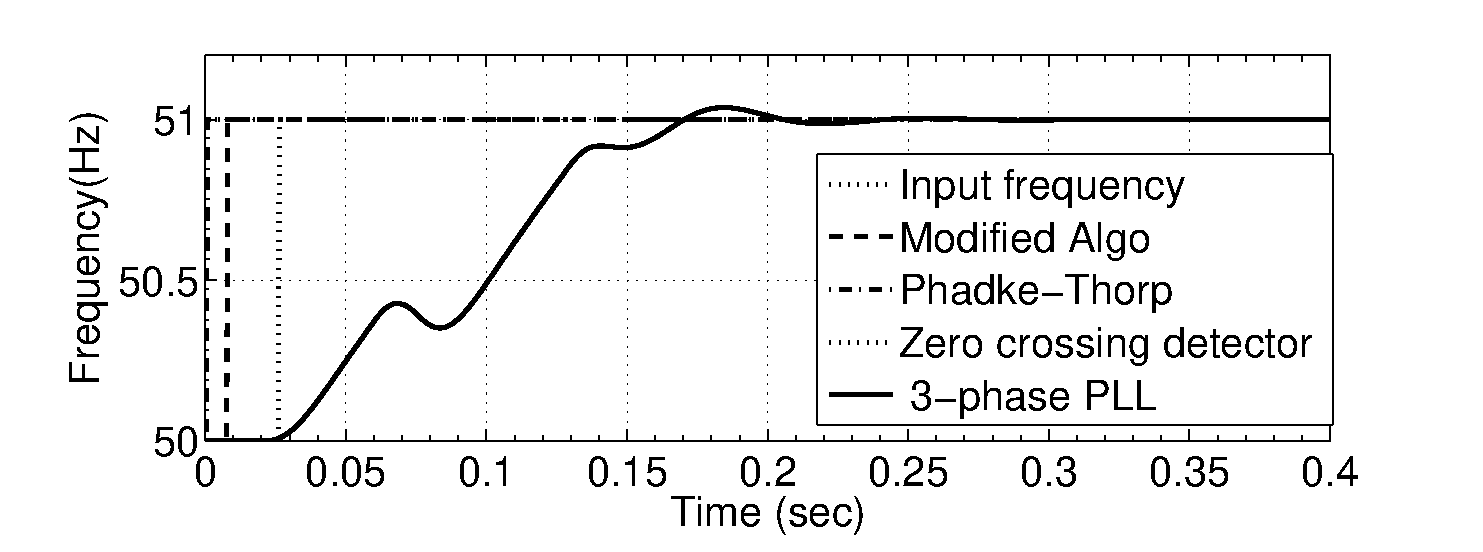
\includegraphics[width=3.0in]{constfreq}
%\caption{Measured frequency for input frequency 51 Hz}
%\label{fig1}
%\end{figure}

\begin{table}[!t]
\caption{Frequency Measurement Results} % title of Table
\centering % used for centering table
\begin{tabular}{c c c c} % centered columns (4 columns)
\hline\hline                        %inserts double horizontal lines
Sr. No. & Frequency & Measured  & \% Error \\ [0.5ex] % inserts table
%heading
\hline % inserts single horizontal line
1 & 47.0 & 47.0033 & +0.0070 \\ % inserting body of the table
2 & 48.0 & 48.0023 & +0.0048 \\
3 & 49.0 & 49.0012  & +0.0024 \\
4 & 49.5 & 49.5006 & +0.0012 \\
5 & 50.0 & 50.0000 & 0.0000 \\
6 & 50.5 & 50.4993 & -0.0014 \\
7 & 51.0 & 50.9986 & -0.0028 \\
8 & 52.0 & 51.9970 & -0.0060 \\
9 & 53.0 & 52.9952 & -0.0091 \\ [1ex] % [1ex] adds vertical space
\hline %inserts single line
\end{tabular}
\label{table_error} % is used to refer this table in the text
\end{table}

\subsubsection{Linearly Increasing Frequency}
\label{linfreq}
The generated three phase signals are as in (\ref{3eqns}),where
%\begin{align*}
%V_a (t) = V_m cos(2\pi ft)\\
%V_b (t) = V_m cos(2\pi ft - 2\pi/3 )\\
%V_c (t) = V_m cos(2\pi ft + 2\pi/3 )
%\end{align*}
\begin{equation}
\label{rate_eqn}
f = \left\{
\begin{array}{ll}
  47 &  0 \leq t < 4 \\
  47 + r*(t-4)  & {4 \leq t <8 }\\
  53 & {8 \leq t <12 }\\
\end{array} \right.
\end{equation}
where,
\newline$r=1.5$ is the rate of change in frequency in Hz/sec.
The results are as shown in \figurename\ref{fig2}

\begin{figure}[!t]
\centering
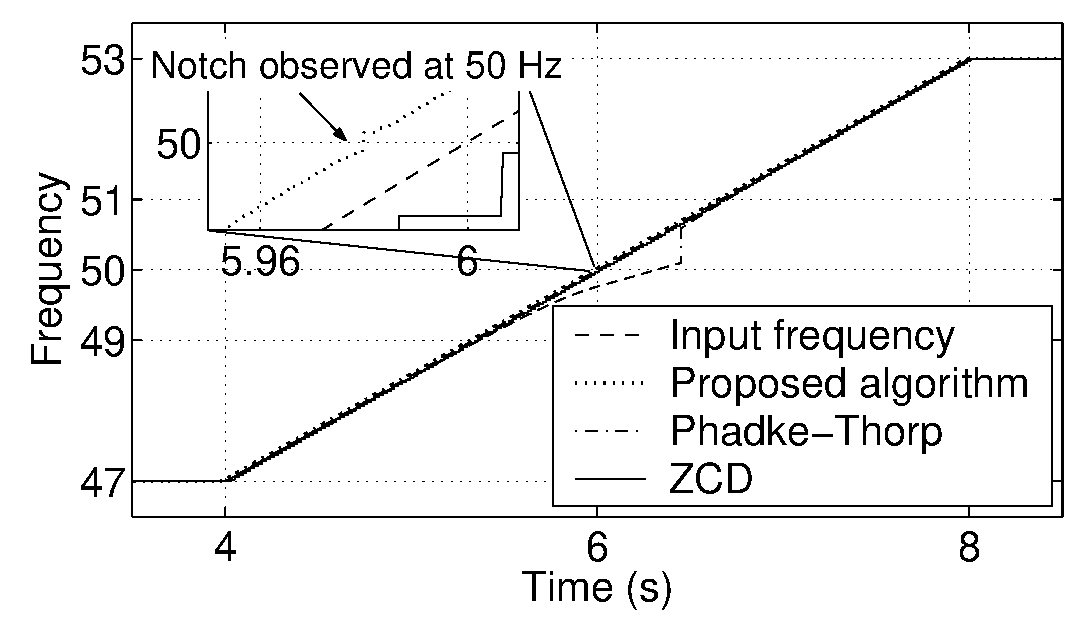
\includegraphics[height=1.6in,width=3in]{kfreq.eps}
\caption{Linearly increasing frequency}
\label{fig2}
\end{figure}

The proposed method and rate-of-change of frequency were applied to case of linearly increasing frequency. In this case the measured frequency faithfully follows the input frequency. The dynamic response of the system in time $4 \leq t < 8$ seconds is approximately linear and takes latching time of 2 cycles ($k$ = 1). To determine whether the deviation of frequency is positive or negative we use Schmitt trigger on the input signal($V_{a}$) and its averaged signal. In a schmitt trigger the sign determination takes place only when the following condition is met. \begin{equation}|V_{a}| \geq V_{th}\label{schmittcondn}\end{equation} In case of linearly increasing frequency that crosses 50 Hz, the magnitude of average signal reduces to zero. The sign determination doesn't take place if $|V_{a}| < V_{th}$ at that instant and get delayed by a few samples till condition in (\ref{schmittcondn}) is met again. This causes a small notch to occur at near about 50 Hz (\figurename \ref{fig2}).The magnitude of this notch is around 0.05 Hz. Reducing the threshold value $V_{th}$ would certainly reduce the notch size but would cause false triggering in noisy signals. A better technique for deviation sign determination would  certainly be a solution to this.
The $r$ estimation algorithm worked as expected for clean signal of increasing frequency. The rate of change of frequency was estimated accurately with delay of 3 cycles: One cyle for the preprocessing of the signal using equations in Section [\ref{rate_estim}] and 2 cycles for frequency estimation algorithm. The \figurename \ref{kestim} illustrates this for $r=1.5$.

\begin{figure}[!t]
\centering
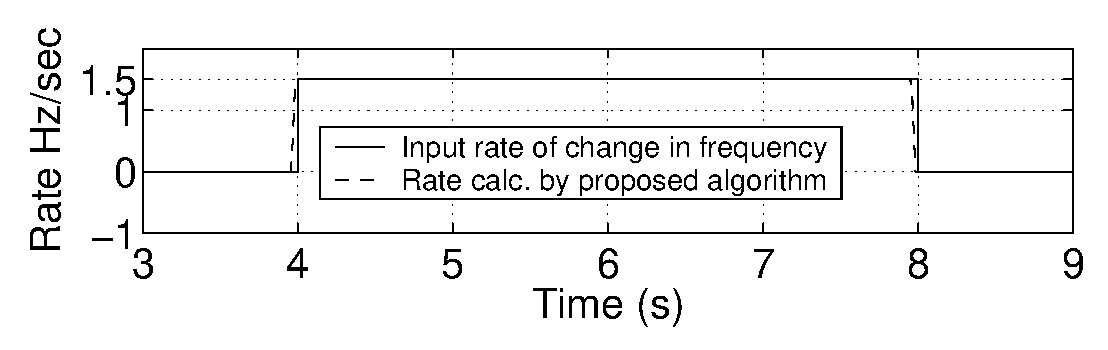
\includegraphics[scale=0.45]{ratekinput}
\caption{Rate-of-change estimation for (\ref{rate_eqn})}
\label{kestim}
\end{figure}



%\begin{figure}[!t]
%\centering
%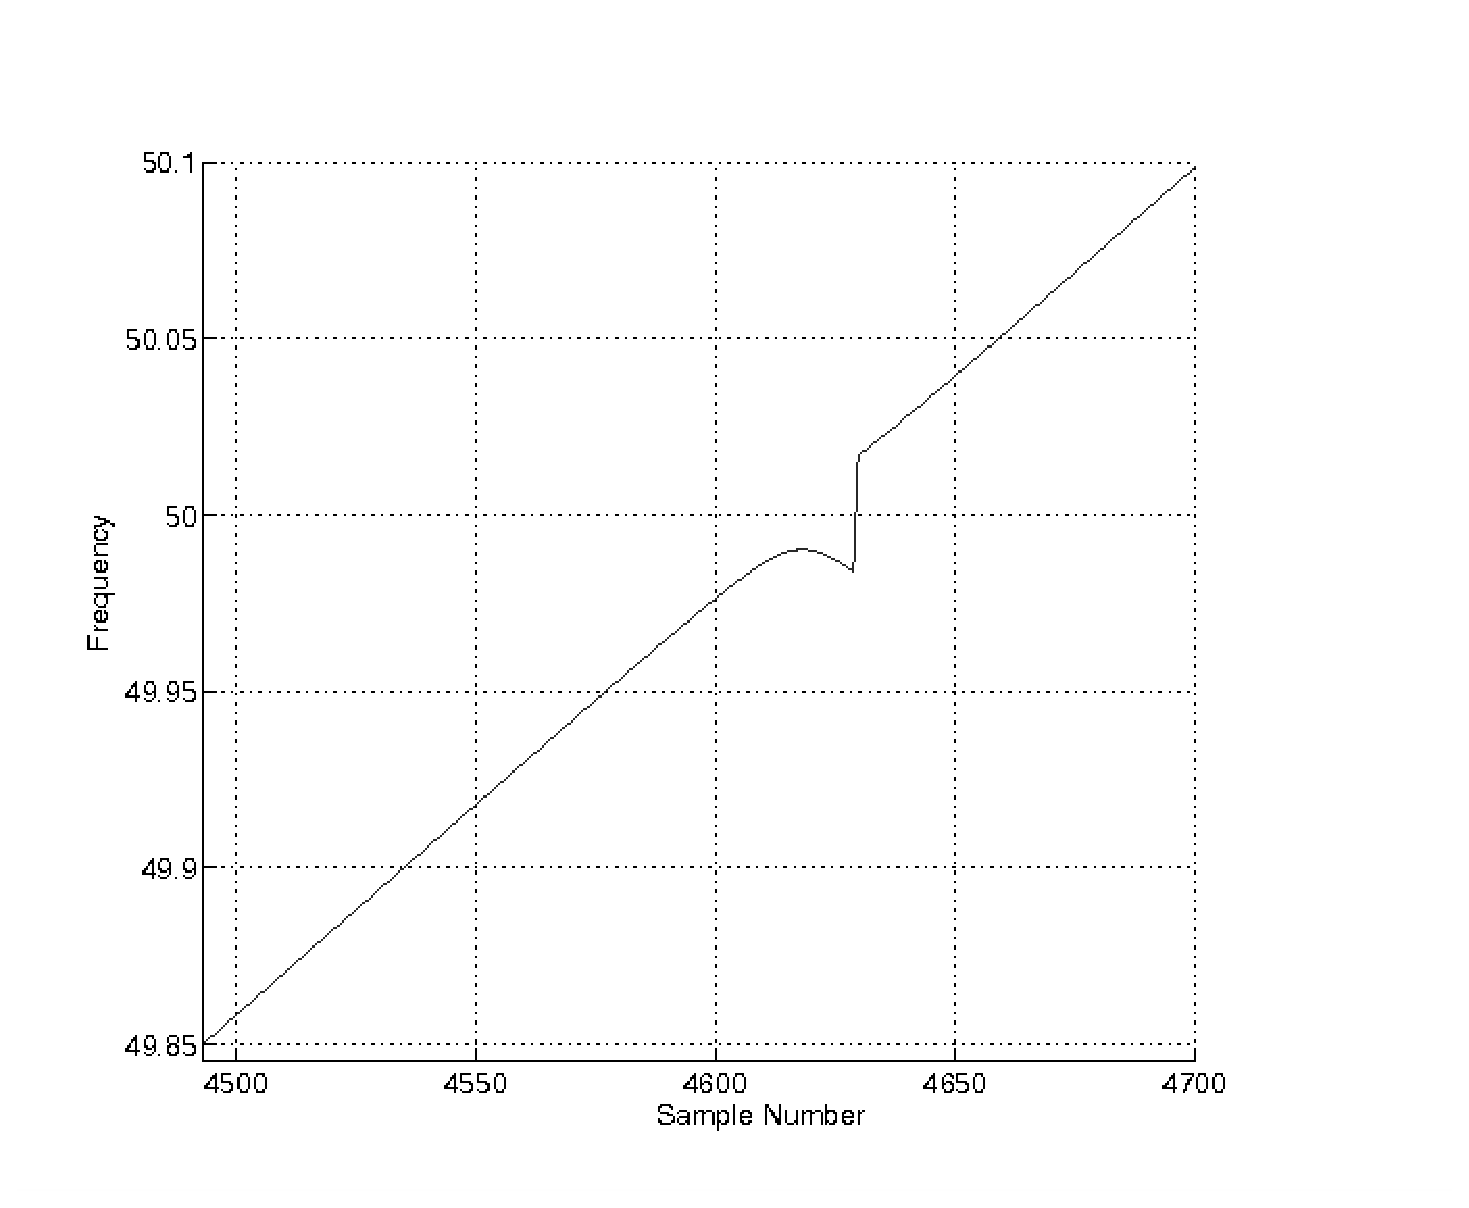
\includegraphics[width=3.0in]{zoomnotch}
%\caption{Observed notch close to 50 Hz }
%\label{zoomnotch}
%\end{figure}

\subsubsection{Non-Linearly Increasing Frequency}
The three phase signals generated are similar to those given in the previous subsection [\ref{linfreq}] except for the fact that the rate of change in frequency $r$ is not constant but varied with time given as follows,
\begin{align}
f &= \left\{
\begin{array}{ll}
  54 &  0 \leq t < 4 \\
  54 + r*(t-4)  & {4 \leq t <8 }\\
  46 & {8 \leq t <12 }\\
\end{array} \right.
\intertext{where,}
r &= \left\{
\begin{array}{ll}
  0 &  0 \leq t < 4 \\
  -2.5 + 0.1*(t-4)*(t-8)  & {4 \leq t <8 }\\
  0 & {8 \leq t <12 }\\
\end{array} \right.
\end{align}
The results are illustrated in the \figurename\ref{nonlinfreq}. Here, we find that the frequency estimated by our proposed algorithm faithfully follows the non-linear input. The instantenous rate of change in frequency is also illustrated in \figurename\ref{nonlink}. The rate $r$ has very high value at $t=8$ seconds due to the fact that there is a step change in the frequency at $t=8$ as seen in the \figurename\ref{nonlinfreq}.
\begin{figure}[!t]
\centering
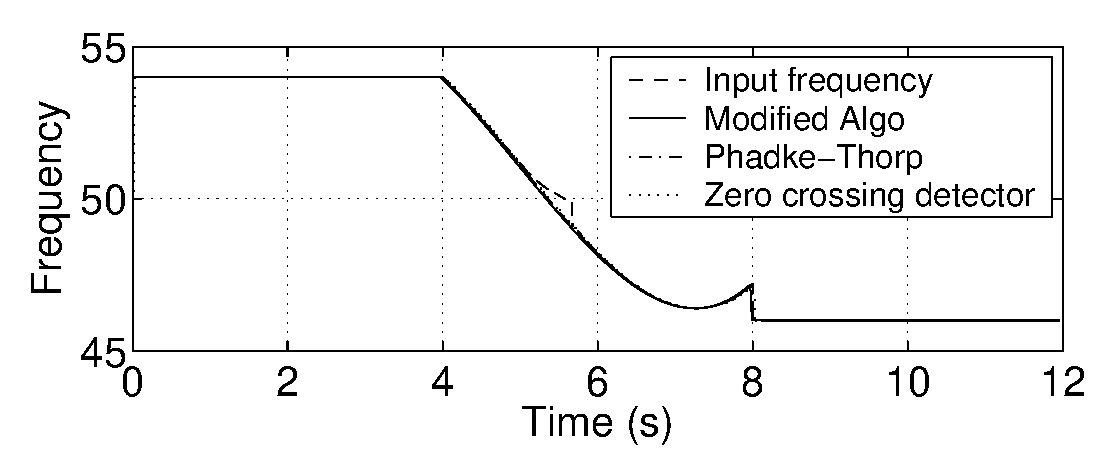
\includegraphics[scale=0.45]{nonlinfreq}
\caption{Frequency plot for non-linear frequency input}
\label{nonlinfreq}
\end{figure}

\begin{figure}[!t]
\centering
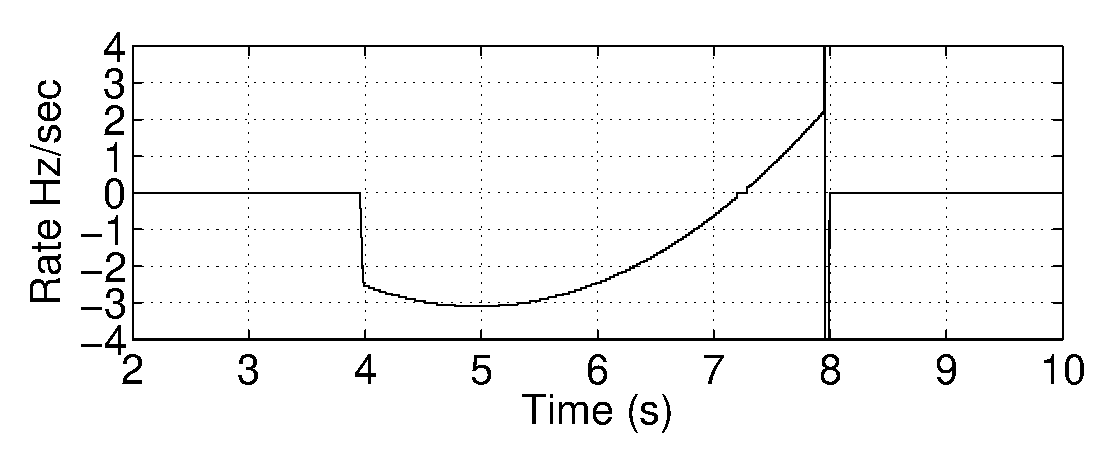
\includegraphics[width=3.0in]{nonlink}
\caption{Rate-of-change estimation for non-linear frequency input}
\label{nonlink}
\end{figure}


\section{Laboratory Experiment}
A laboratory experiment was performed to carry out a performance study of the proposed method using real voltage samples. \figurename \ref{testbed} below outlines the experimental setup for collection of voltage data samples. A synchronous generator at no-load coupled with a DC motor was used to generate balanced three-phase voltage signals with constant and varying frequency. Three-phase voltages were signal conditioned and sampled using a data-acquisition card with constant sampling rate of $N$=50 samples per cycle and were recorded on the computer.The ADC resolution used was 10-bit. Simulations were carried out in MATLAB with collected data and results obtained were then compared to other methods: Phadke-Thorp method \cite{phadkethorp},Phase Locked Loop, Zero-crossing detector.

\begin{figure}[!t]
\centering
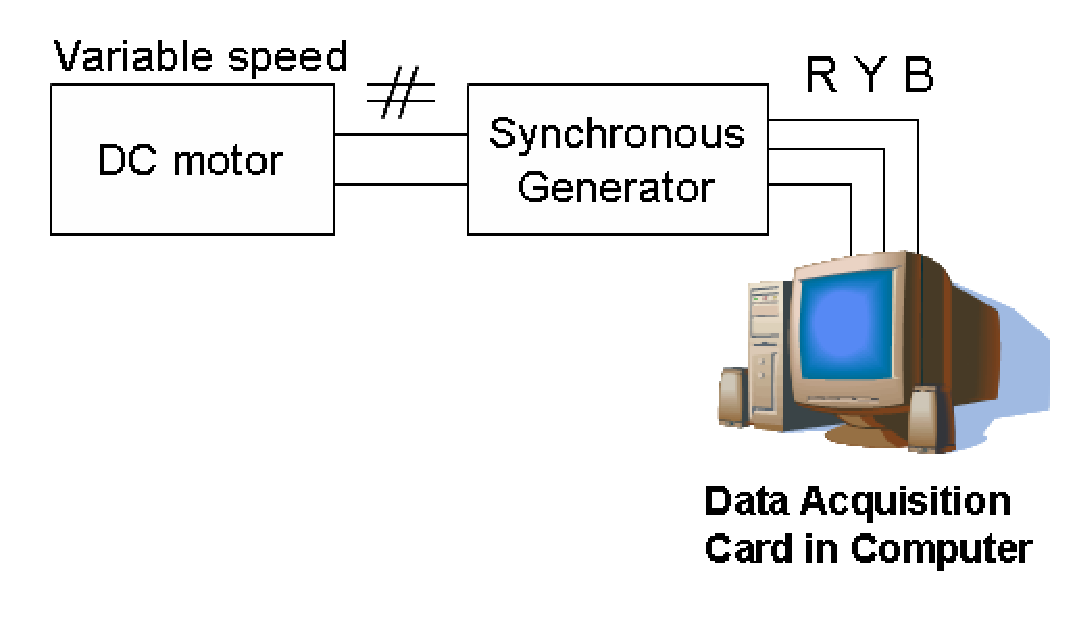
\includegraphics[height=1.3in,width=3.0in]{testbed}
\caption{Experiment setup}
\label{testbed}
\end{figure}

\begin{figure}[!t]
\centering
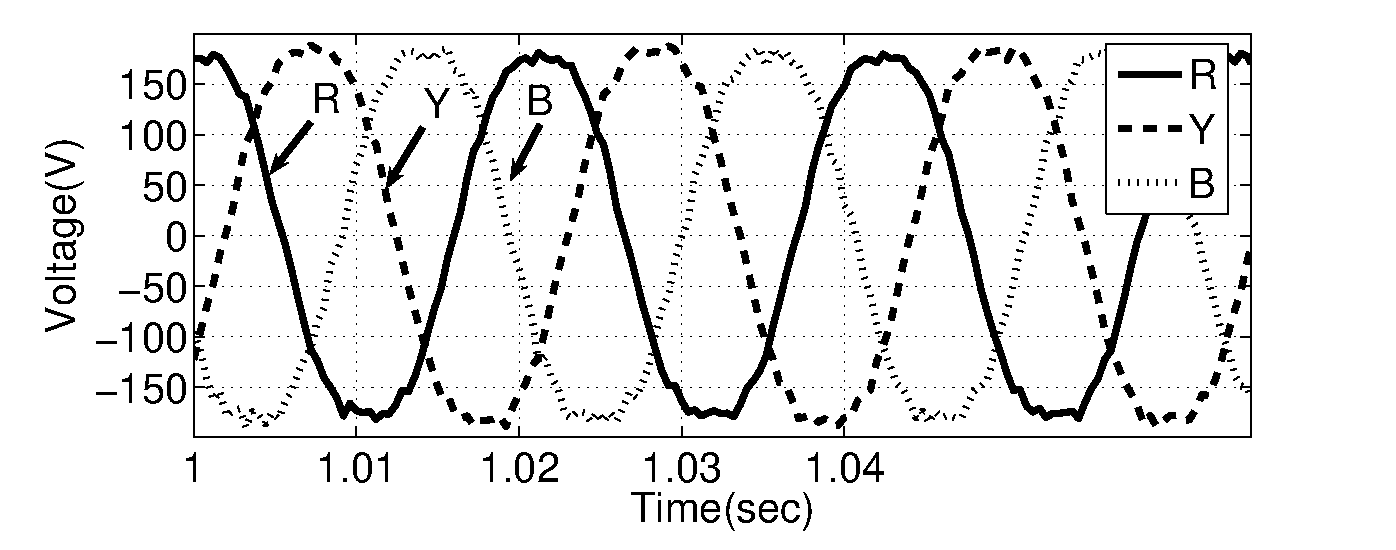
\includegraphics[width=3.0in]{rybvolt}
\caption{Three phase voltages}
\label{rybvolt}
\end{figure}

\subsection{Constant Frequency}
Steady state response of algorithm to generator generated signals(\figurename \ref{rybvolt}) is shown in \figurename \ref{fig:prop}. Three other methods were used for a accuracy comparison of the measured frequency. \figurename\ref{fig:pt} is the phasor method of Phadke-Thorp \cite{phadkethorp} which used DFT as nominal frequency $f_{0}$ and then measures the time taken for phasor to rotate by $\theta$ radians ($\theta$=0.5 rad in this case). This method used a sum the previous samples phase-change and counts the time taken to complete $\theta$=0.5 rad. Hence the response is quite steady and smoothed out. \figurename \ref{fig:pll} is a response to a tuned Phase Locked Loop, the response is as expected steady by sight oscillatory. And finally as zero-crossing detector implementation is shown in \figurename \ref{fig:zcd}. All these and results for several other frequencies have been summarized in table \ref{table_rybfreq}. Generator speed measured by means of a tachometer and calculated frequency by using Eqn. \ref{gen_formula}.
\begin{equation}
f=NP/120
 \label{gen_formula}
\end{equation}
where $N$=generator speed($rpm$), $P$= number of poles, $f$= frequency($Hz$).

Increasing the window size over $k$ cycles where $k = 1,2,3,4.$ and using sensitivity enhancement technique of section \ref{sens_enhance}, the averaging effect is clearly seen in \figurename\ref{diffkvalues}. The oscillations in frequency have reduced but at the expense of added delay ($2k$ cycles.). Above $k=4$ cycles tthe technique overestimates the frequency value and hence k is restricted at $k=4$ cycles.
\begin{figure}[!t]
\centering
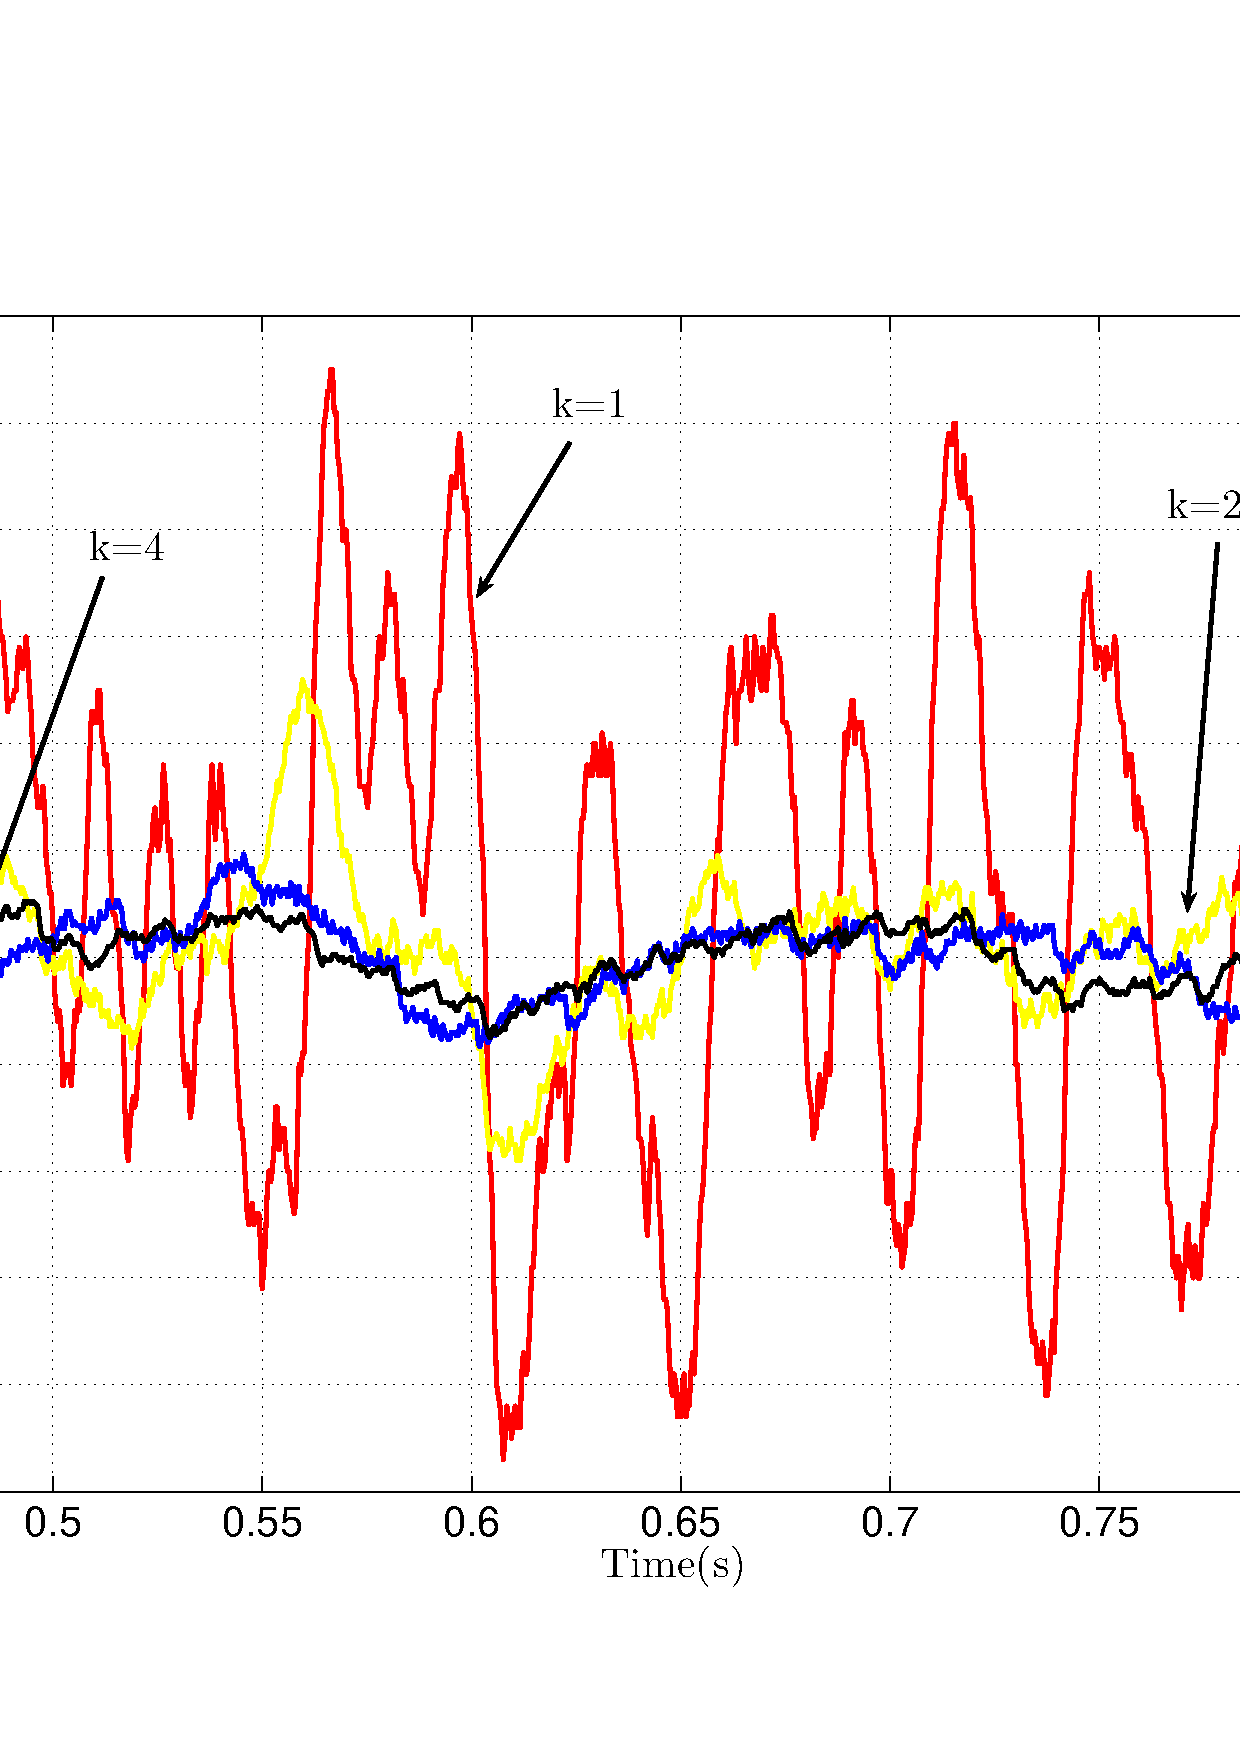
\includegraphics[width=3.0in]{diffkvalues}
\caption{Response for different $k$ values}
\label{diffkvalues}
\end{figure}


\begin{table}[!t]
\caption{Frequency Measurement Results For Generator Averaged Over One sec.} % title of Table
\centering % used for centering table
\begin{tabular}{c c c c c c} % centered columns (6 columns)
\hline\hline                        %inserts double horizontal lines
Gen. & Calculated & Proposed & Phadke- & PLL & Zero- \\ % inserts table
RPM & frequency & method & Thorp & detector &  cross. \\ [0.5ex]
%heading
\hline % inserts single horizontal line
1312 & 43.7333 & 43.7579 & 43.7500 & 43.7525 & 43.7520\\ % inserting body of the table
1337 & 44.5667 & 44.5941 & 44.5584 & 44.5885 & 44.5893\\
1346 & 44.8667 & 44.8998 & 44.8637 & 44.8951 & 44.8987\\
1369 & 45.6333 & 45.6677 & 45.6363 & 45.6623 & 45.6619\\
1386 & 46.2000 & 46.1463 & 46.1376 & 46.1429 & 46.1406\\
1398 & 46.6000 & 46.7203 & 46.7598 & 46.7173 & 46.7181\\
1423 & 47.4333 & 47.4143 & 47.4044 & 47.4124 & 47.4121\\
1450 & 48.3333 & 48.1893 & 48.1727 & 48.1869 & 48.1896\\
1467 & 48.9000 & 48.9245 & 48.9201 & 48.9233 & 48.9238\\
1479 & 49.3000 & 49.3213 & 49.3383 & 49.3214 & 49.3231\\
1490 & 49.6667 & 49.6921 & 49.7074 & 49.6931 & 49.6911\\
1501 & 50.0333 & 50.1754 & 50.2032 & 50.1875 & 50.1887\\
1520 & 50.6667 & 50.6036 & 50.6323 & 50.6038 & 50.6046\\
1539 & 51.3000 & 51.2378 & 51.2096 & 51.2386 & 51.2398\\
1560 & 52.0000 & 51.9918 & 51.9967 & 51.9950 & 51.9937\\
1590 & 53.0000 & 53.0364 & 53.0351 & 53.0408 & 53.0415\\
1602 & 53.4000 & 53.4046 & 53.4107 & 53.4098 & 53.4146\\
1622 & 54.0667 & 54.0870 & 54.0679 & 54.0934 & 54.0965\\ [1ex] % [1ex] adds vertical space
\hline %inserts single line
\end{tabular}
\label{table_rybfreq} % is used to refer this table in the text
\end{table}

\begin{figure}[!t]
  \centering
    \subfigure[Proposed method with $k=1$]{\label{fig:prop}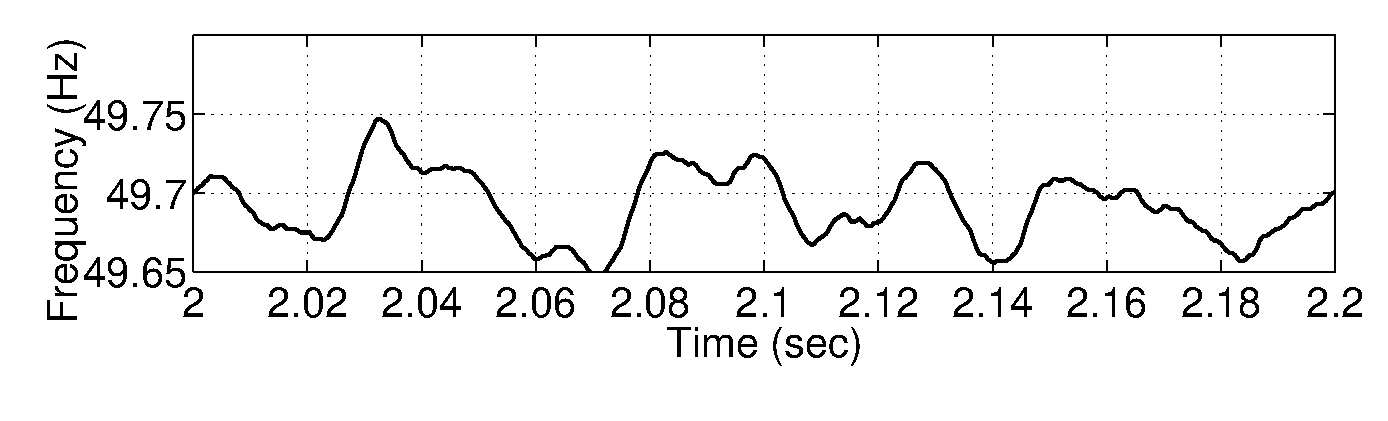
\includegraphics[width=3.0in]{prop}}\\
    \subfigure[Phadke-Thorp method]{\label{fig:pt}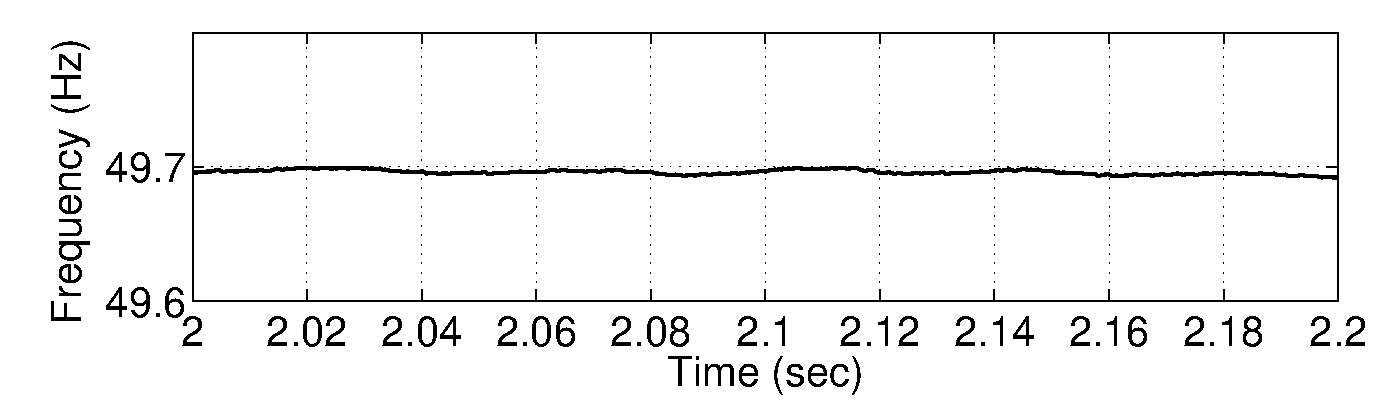
\includegraphics[width=3.0in]{pt}} \\
    \subfigure[Phase Locked Loop]{\label{fig:pll}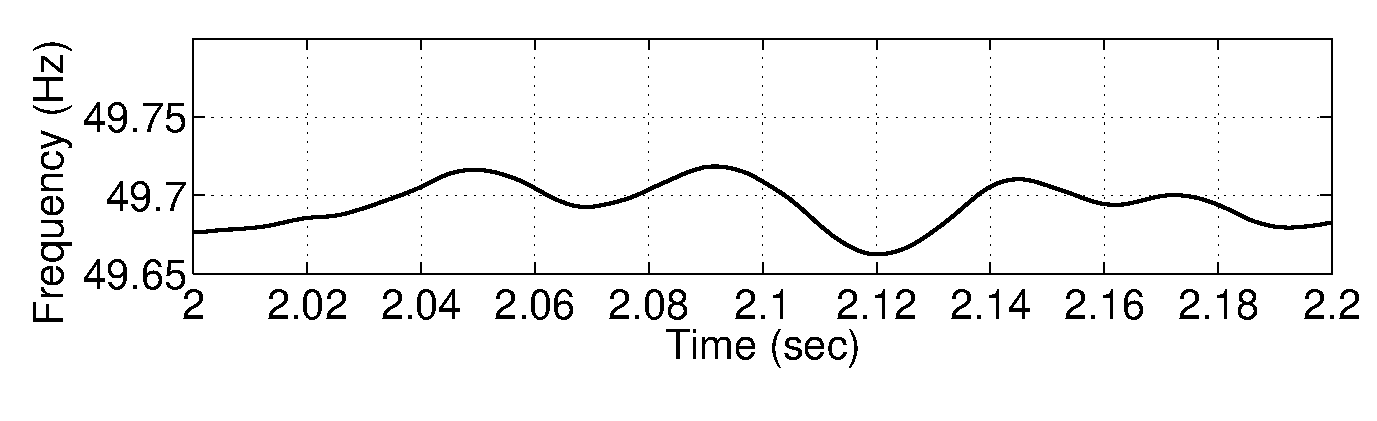
\includegraphics[width=3.0in]{pll}} \\
    \subfigure[Zero-crossing detector]{\label{fig:zcd}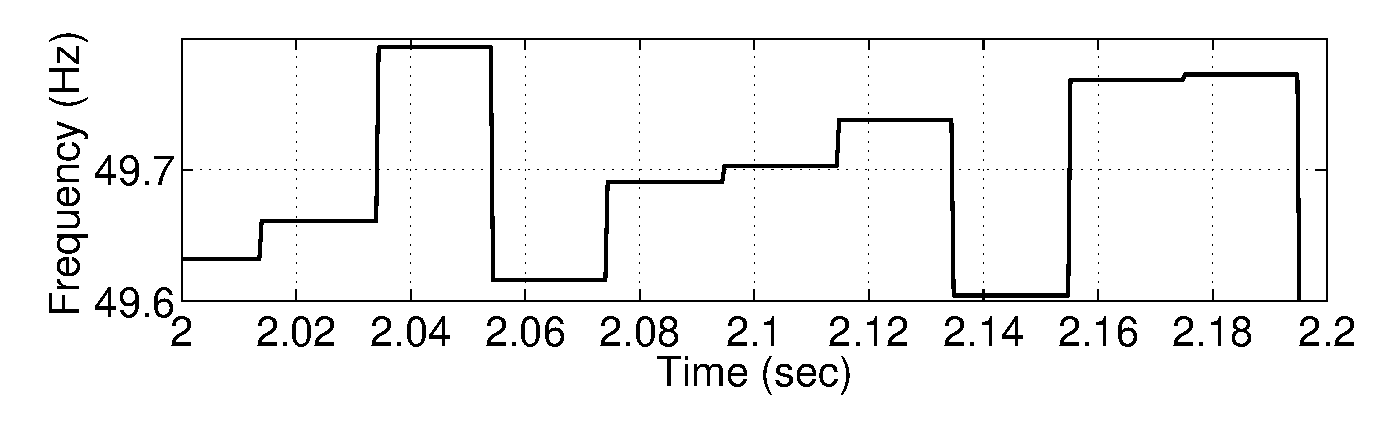
\includegraphics[width=3.0in]{zcd}}\\
  \caption{Plot of frequency estimated by various frequency detection algorithms using generator data corresponding to 48.9 Hz}
  \label{fig:edge}
\end{figure}
% \begin{figure}[!ht]
% \begin{center}
% 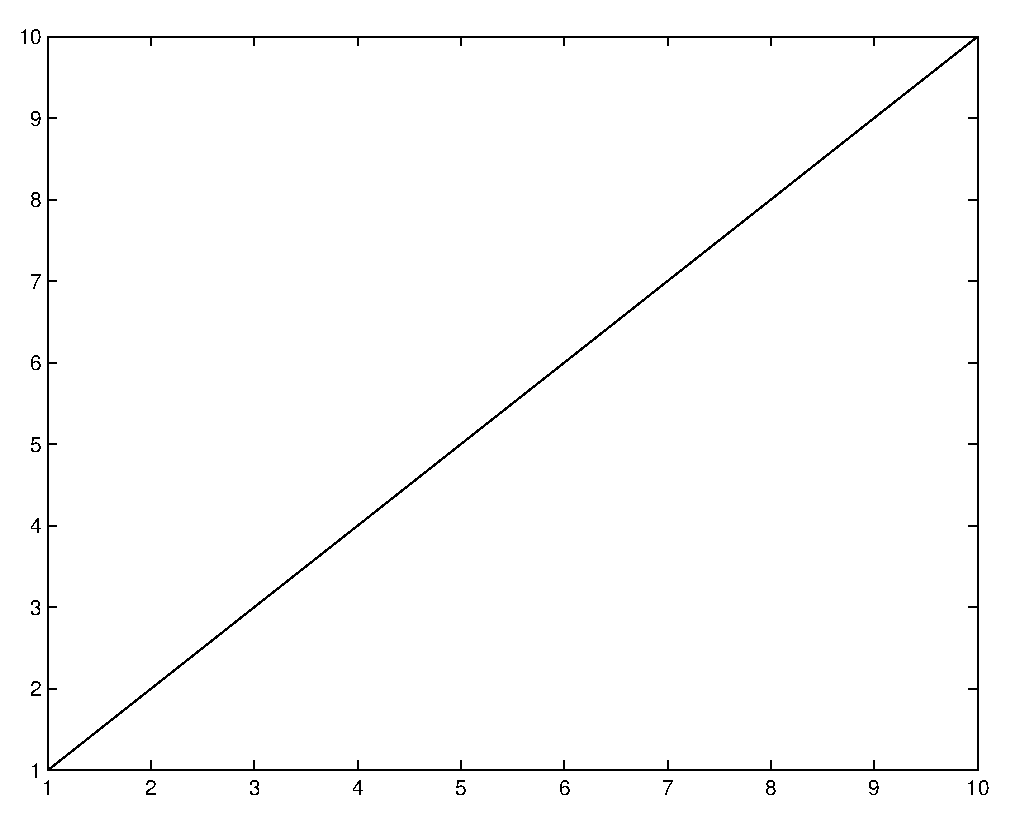
\includegraphics[scale=0.3]{fig}
% \caption{Constant frequency graph for RYB input}
% \label{rybconstfreq}
% \end{center}
% \end{figure}
\subsection{Linearly Varying Frequency}
For simulating linearly varying frequency, the resistance in series with the field winding of DC motor was varied. The variation was done manually for approximately linear output. A linear change in the speed of the synchronous generator is assumed on account of its rotor inertia. It is evident from the \figurename\ref{ryblinearfreq} that the frequency estimated by Phadke-Thorp method\cite{phadkethorp} is not accurate around 50Hz. The frequency estimated by PLL is used as the reference in this range. The measured frequency by the proposed algorithm follows the input quite accurately estimated by the algorithm.
The rate-of-change of frequency measured for the \figurename\ref{ryblinearfreq}. For different values of $k$ ($k=1,2,3,4.$) the measured value of rate of change of frequency was found to be close to accurate with higher values of $k$. This is shown in \figurename\ref{rybKestim}. The algorithm gives fair amount of qualitative information regarding the change of frequency.
%  The rate of change of frequency algorithm although couldn't measure this as it was found quite sensitive to the noise in the signal. The schmitt trigger also gave some problems here due to bad signals. \figurename\ref{rybKestim} shows this. One reason for this might be the blue phase in the average signal which is not balanced and seems to ride on a low frequency signal. See \figurename \ref{rybavgKestim}. But this isn't seen in the orignal signal from the generator which is clean.
\begin{figure}[!t]
 \centering
 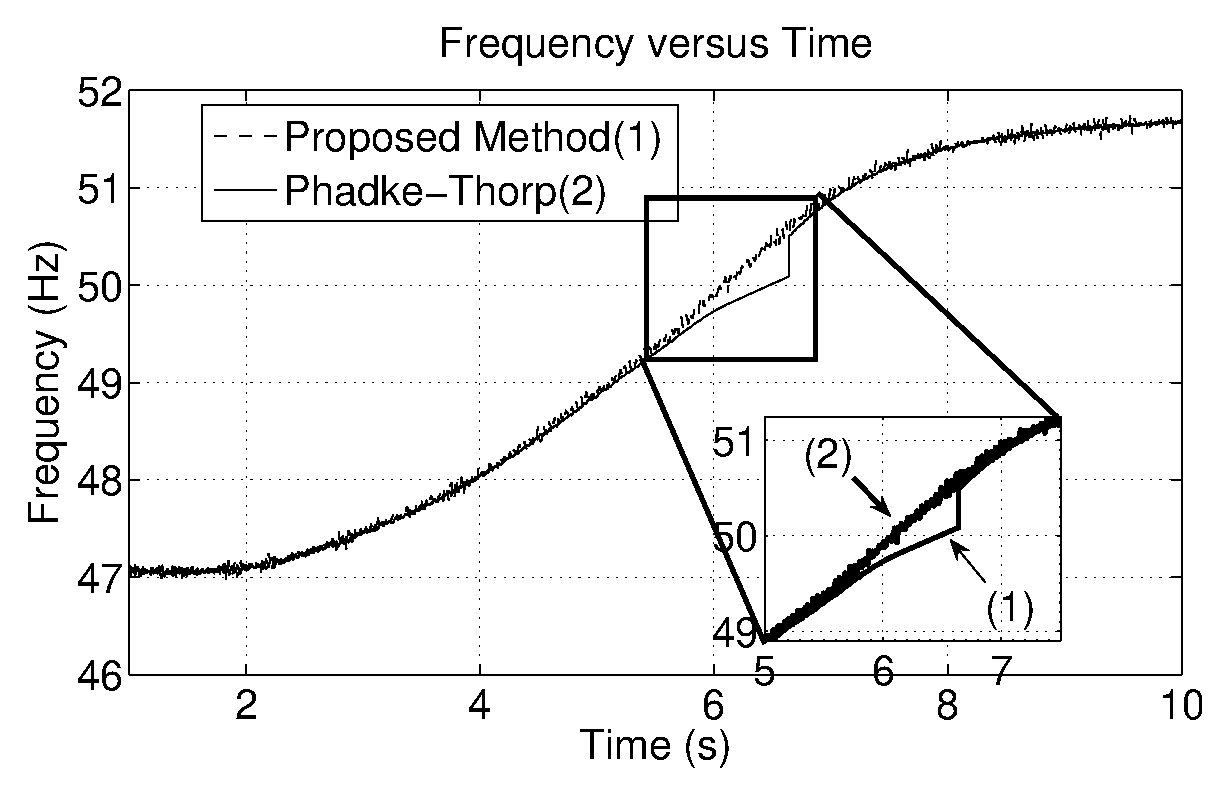
\includegraphics[width=3.0in]{ryblinearfreq}
 \caption{Linear varying frequency of generator}
 \label{ryblinearfreq}
 \end{figure}

\begin{figure}[!t]
 \centering
 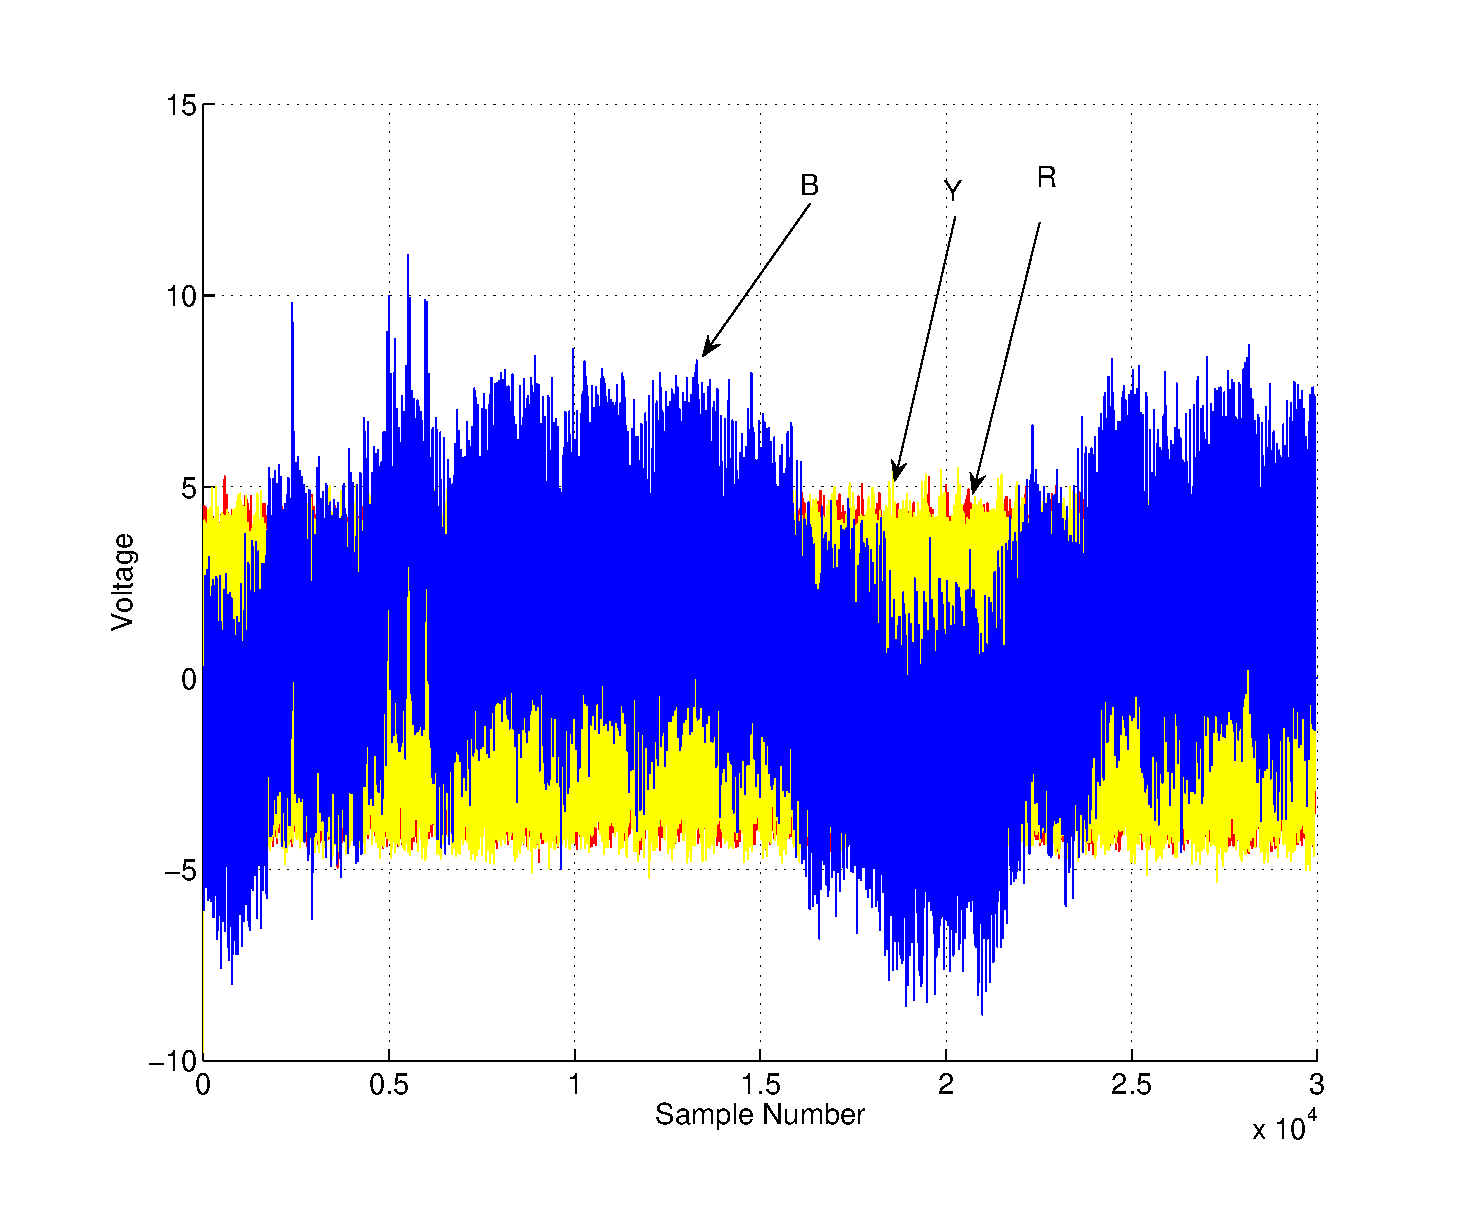
\includegraphics[width=3.0in]{rybavgkestim}
 \caption{Averaged signal of the generator}
 \label{rybavgKestim}
 \end{figure}
%
 \begin{figure}[!t]
   \centering
     \subfigure[$k=1$]{\label{fig:k1}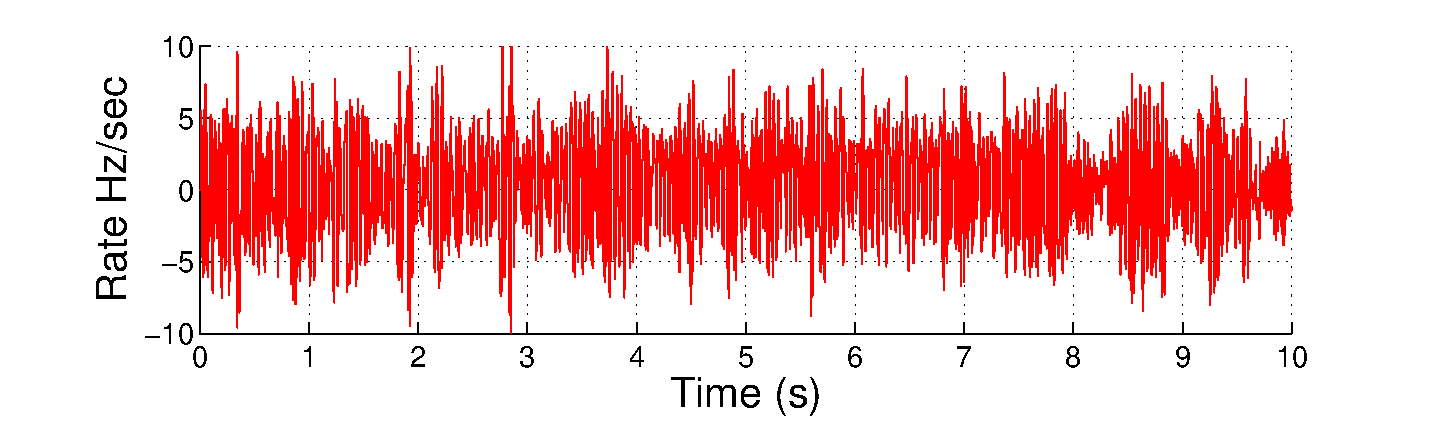
\includegraphics[width=3.0in]{k1}} \\
    \subfigure[$k=2$]{\label{fig:k2}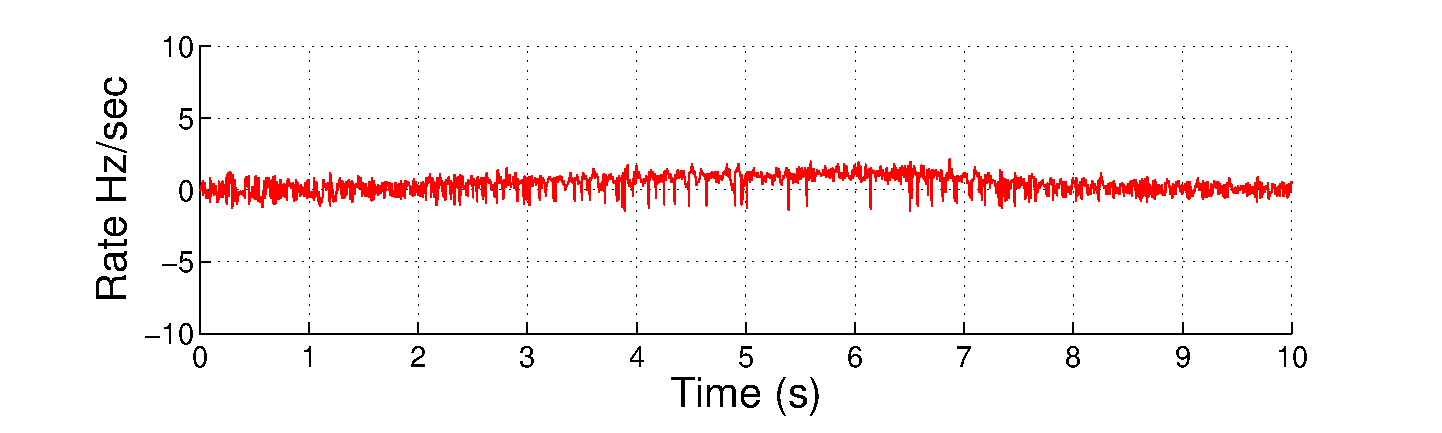
\includegraphics[width=3.0in]{k2}} \\
    \subfigure[$k=3$]{\label{fig:k3}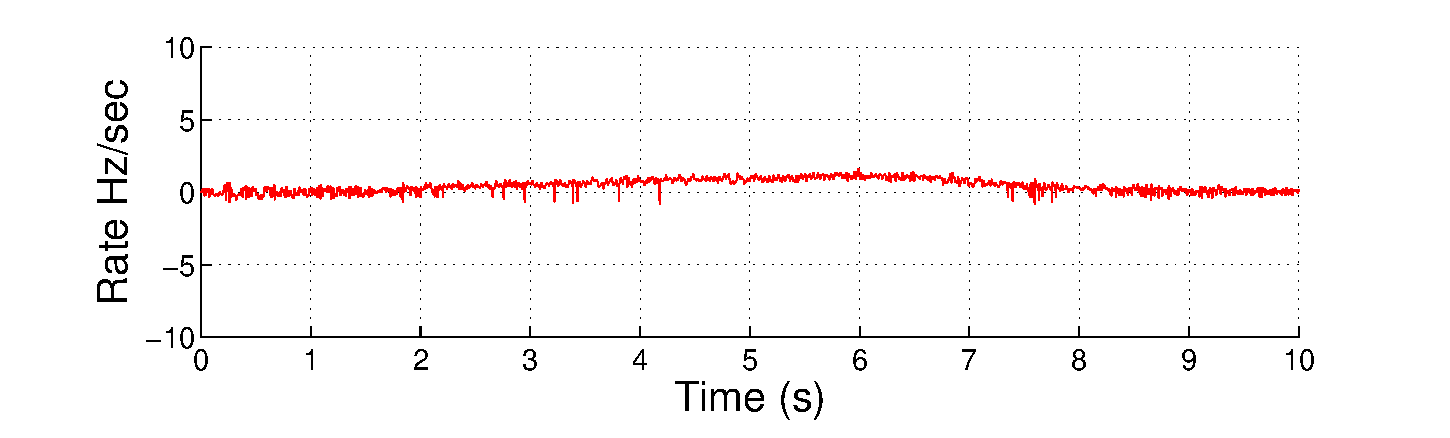
\includegraphics[width=3.0in]{k3}} \\
     \subfigure[$k=4$]{\label{fig:k4}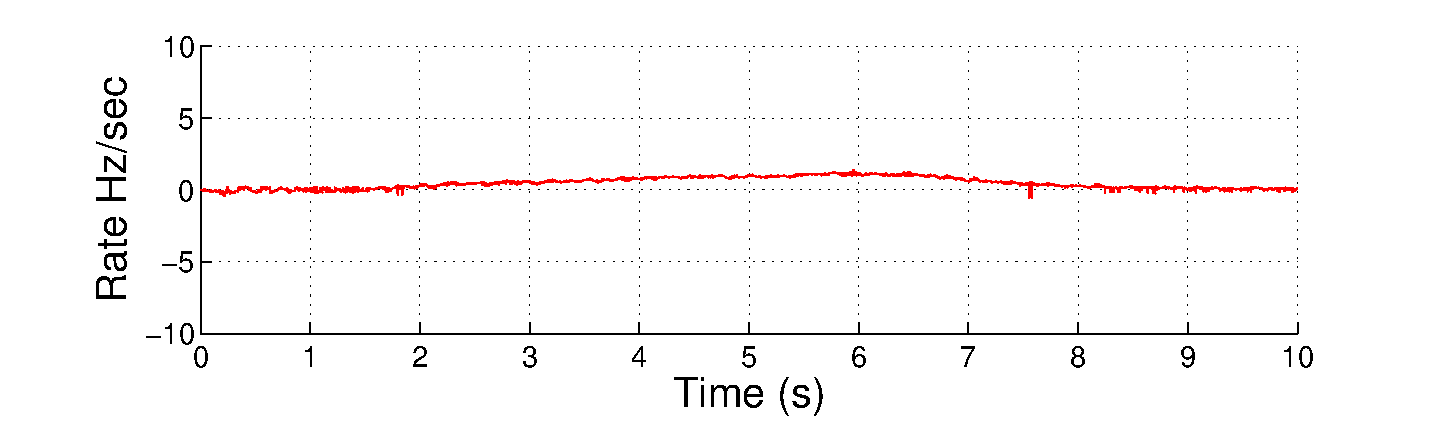
\includegraphics[width=3.0in]{k4}} \\

   \caption{Rate of change of frequency estimation for generator signals}
   \label{rybKestim}
 \end{figure}

\subsection{System Frequency}
As a verification, samples collected from three-phase system supply were fed to the algorithm. The results obtained are as shown in the \figurename \ref{system_freq}. The frequency measured is compared with phasor method of Phadke-Thorp \cite{phadkethorp}. The measured frequency is quite close to actual frequency measured by phasor method of Phadke-Thorp.
 \begin{figure}[!t]
 \centering
 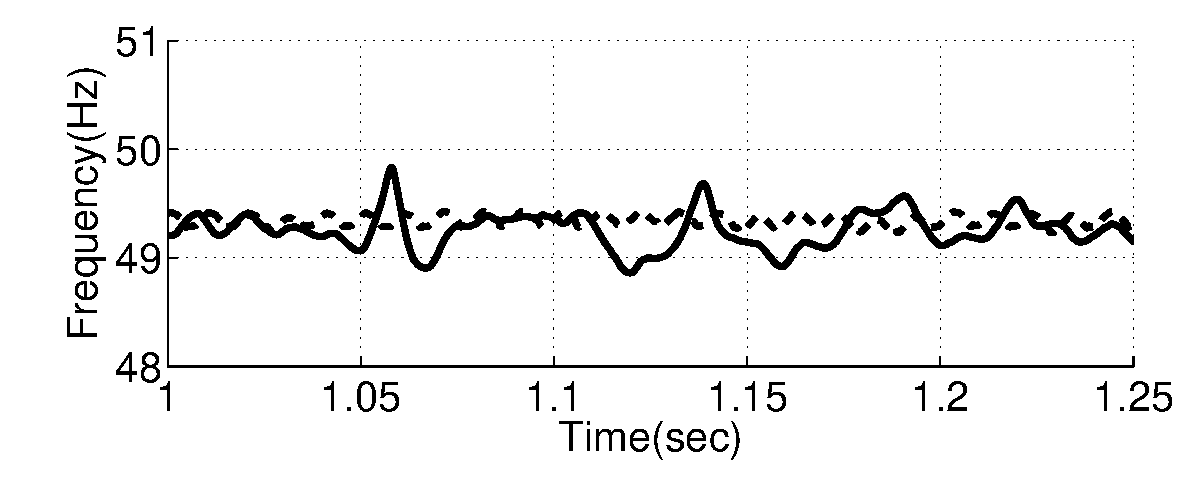
\includegraphics[width=3.0in]{system_freq}
 \caption{Power system frequency $(k=1)$}
 \label{system_freq}
 \end{figure}

%\subsection{Things we tried}Modification:- Double averaging the original signal and subtracting a shifted ( by $\pi/2$ ) form of it from the orignal average signal to reduce noise .Output- This thing didn't work in generator signal for any shift.Modification:- Taking average after sequence components so that noise in the signal is reduced.Thus, this involves taking DFT twice over the same signal.Output- Gave better results but introduces a total 4 cycles delay in the output.

